\documentclass[11pt]{aghdpl}
% \documentclass[en,11pt]{aghdpl}  % praca w języku angielskim
\usepackage[polish]{babel}
%\usepackage[english]{babel}
\usepackage[utf8]{inputenc}

% dodatkowe pakiety
\usepackage{enumerate}
\usepackage{listings}
\usepackage{amsmath}
\usepackage{amsfonts}
\usepackage{tabularx}
\lstloadlanguages{TeX}

\lstset{
  literate={ą}{{\k{a}}}1
           {ć}{{\'c}}1
           {ę}{{\k{e}}}1
           {ó}{{\'o}}1
           {ń}{{\'n}}1
           {ł}{{\l{}}}1
           {ś}{{\'s}}1
           {ź}{{\'z}}1
           {ż}{{\.z}}1
           {Ą}{{\k{A}}}1
           {Ć}{{\'C}}1
           {Ę}{{\k{E}}}1
           {Ó}{{\'O}}1
           {Ń}{{\'N}}1
           {Ł}{{\L{}}}1
           {Ś}{{\'S}}1
           {Ź}{{\'Z}}1
           {Ż}{{\.Z}}1
}

%---------------------------------------------------------------------------

\author{Szymon Sobański}
\shortauthor{S. Sobański}

\titlePL{Kontekstowa konsolidacja i agregacja informacji ze stron internetowych z wykorzystaniem asocjacyjnych struktur AGDS w celu optymalizacji ich przetwarzania.}
\titleEN{}

\shorttitlePL{Kontekstowa konsolidacja i agregacja informacji ze stron internetowych z wykorzystaniem asocjacyjnych struktur AGDS w celu optymalizacji ich przetwarzania.} % skrócona wersja tytułu jeśli jest bardzo długi
\shorttitleEN{Thesis in \LaTeX}

\thesistype{Praca dyplomowa inżynierska}
%\thesistype{Master of Science Thesis}

\supervisor{dr inż. Adrian Horzyk}
%\supervisor{Marcin Szpyrka PhD, DSc}

\degreeprogramme{Automatyka i Robotyka}
%\degreeprogramme{Computer Science}

\date{2014}

\department{Katedra Automatyki}
%\department{Department of Applied Computer Science}

\faculty{Wydział Elektrotechniki, Automatyki,\protect\\[-1mm] Informatyki i Inżynierii Biomedycznej}
%\faculty{Faculty of Electrical Engineering, Automatics, Computer Science and Biomedical Engineering}

\acknowledgements{Serdecznie dziękuję \dots tu ciąg dalszych podziękowań np. dla promotora, żony, sąsiada itp.}


\setlength{\cftsecnumwidth}{10mm}

%---------------------------------------------------------------------------
\newtheorem{definicja}{Definicja}

\begin{document}

\titlepages

\tableofcontents
\clearpage

\chapter{Wprowadzenie}
\label{cha:wprowadzenie}

Wraz z rozpowszechnieniem dostępu do Internetu, można zauważyć zwiększenie ilości produkowanych informacji. Jak wynika z przygotowanego przez organizację IDC raportu, między latami 2009, a 2020, przewiduje się 44 krotny wzrost ilości danych dostępnych w sieci \cite{DigUni}. Jednym z najbardziej odczuwalnych skutków wzrostu ilości i dostępności danych, dotykający również przedsiębiorstwa, jest tzw. \emph{Information Overload}, czyli nadmiar czynników branych pod uwagę  w różnych procesach decyzyjnych. Wpływa to na obniżenie dynamiki, innowacyjności i konkurencyjności na rynku i ma wyraźny negatywny wpływ na gospodarkę \cite{InfOver}.

Z drugiej strony, łatwo dostępne i zróżnicowane dane mogą służyć jako podstawa rozwoju, dając przede wszystkim dostęp do ogromnej bazy wiedzy zgromadzonej w sieci, jak i umożliwiając przedsiębiorcom zdobycie wiedzy o kosnumentach, łatwiejsze badanie rynku i dostosowanie oferowanych usług do potrzeb klientów \cite[s. 1-26]{DMining}.

Głównym problemem zatem pozostaje kwestia sposobu porządkowania i filtracji dostępnych danych, w celu ich wykorzystania. Klasycznym przykładem aplikacji służacej do tego celu jest \emph{wyszukiwarka~internetowa} - witryna dostępna w sieci, która umożliwia przeszukiwanie Internetu pod kątem wprowadzanych przez użytkownika zapytań.

%---------------------------------------------------------------------------

\section{Cele pracy}
\label{sec:celePracy}

Celem poniższej pracy jest zaproponowanie rozwiązania porządkującego dane pochodzące z sieci internetowej i przechowującego je w postaci grafu asocjacyjnego - AGDS \cite[s. 112-117]{Horzyk}.

Poruszone zostają kwestie budowy oprogramowania eksplorującego sieć i pobierającego treść stron, przechowywania tak zdobytych informacji i przetwarzania ich w celu umieszczenia w grafie. Przedstawione zostają argumenty przemawiające za takim rozwiązaniem, poddana dyskusji zostaje różnica pomiędzy proponowanym podejściem, a rozwiązaniami wiodącymi obecnie prym w zastosowaniach komercyjnych.
%
%Zaprezentowany  zostaje algorytm budowania sieci AGDS, poruszone zostają szczegóły implementacyjne poszczególnych elementów składowych aplikacji. Wyjaśnia się jej architekturę i zabiegi zastosowane w celu zwiększenia modułowości i separacji kodu, opisane zostają perspektywy rozwoju. Przybliża się również 

Ponadto zaproponowano wykorzystanie tak przechowywanych danych do budowy prostej asocjacyjnej wyszukiwarki internetowej, opartej o neuroasocjacyjne grafy wiedzy ANAKG\cite[s. 223-244]{Horzyk}. 


%---------------------------------------------------------------------------

\section{Zawartość pracy}
\label{sec:zawartoscPracy}

W rodziale~\ref{cha:pozyskiwanieTresci} przedstawiono podstawowe informacje dotyczące pozyskiwania danych z witryn internetowych. Zilustrowane są podstawowe wymagania stawiane przed oprogramowaniem trawersującym sieć, tzw. \emph{crawlerem}, poruszone są kwestie wydajności, poprawnej implementacji, oraz opisane są względy etyczne, którymi należy się kierować przy korzystaniu z takiego oprogramowania.

Rozdział~\ref{cha:przetwarzanieDanych} ma na celu opisanie problemów dotyczących ekstrakcji danych z dokumentu HTML. Zawiera on krótki opis formatu, przestawia jego zastowania i wyjaśnia, dlaczego poprawne uzyskiwanie informacji ze źródeł stron internetowych nie jest zadaniem trywialnym. Ponadto, zilustrowane są różne podejścia do parsowania zawartości dokumentów HTML, jak i przedstawiona jest pokrótce nomenklatura różnych typów stron, w kontekście wyszukiwarek internetowych.

Rozdział~\ref{cha:budowaGrafu} prezentuje podstawowe informacje o asocjacyjnych grafach AGDS. Wyjaśnia powód zainteresowania takimi strukturami, wskazuje na ich zalety, przedstawia sposób tworzenia struktur i przytacza przykładowe grafy stworzone za pomocą oprogramowania będącego częścią projektu. Stara się również przedstawić konsekwencje sposobów budowy grafu i możliwość uzyskiwania informacji, zawartych w takich strukturach.

Następnie, w rozdziale~\ref{cha:implementacja}, opisane są szczegóły implementacyjne aplikacji realizującej cele pracy. Wyjaśnione są szczegóły architektury, przytoczone zalety wybranch technologii, poruszony jest temat wydajności oprogramowania. Przedstawione jest również działanie całej aplikacji, wraz z wyjaśnieniem założeń testowych.

Rozdział \ref{cha:wyszukiwarka} przedstawia aplikację wykorzystującą graf AGDS i zbudowaną w oparciu o niego sieć neuronową ANAKG do wyszukiwania stron internetowych. Przedstawia on podstawowe założenia stojące za budową sieci ANAKG, algorytm jej pobudzania, jak i sposób interpretacji wyników. Podjęta jest również próba ilustracji odpowiedzi sieci dla różnych parametrów symulacji.



















\chapter{Pozyskiwanie treści z Internetu}
\label{cha:pozyskiwanieTresci}

Pozyskiwaniem treści z sieci zajmuje się grupa oprogramowania nazywana sieciowymi pająkami(ang. \emph{web crawlers}, \emph{web spiders}) lub sieciowymi robotami(ang. \emph{web robots}). Danymi wejściowymi jest zazwyczaj grupa stron, a właściwie adresów URL, nazywana \emph{seedem} \cite{webCrawling}. Ich zadanie zazwyczaj nie ogranicza się do pobrania jednej strony, ale do trawersowania całej sieci, bądź w celu pozyskania konkretnych informacji, bądź w celu jej eksploracji. Przy czym w związku z ilością danych dostępnych w Internecie zazwyczaj zakłada się pewne filtry i ograniczenia, w celu zwiększenia efektywności robota i zwiększenia szans na odwiedziny najbardziej wartościowych, dla danego zastosowania, stron.

W związku z dynamiczną naturą Internetu, koniecznym jest ciągłe odświeżanie posiadanych już informacji, poszukiwanie nowych stron i ew. eliminacja witryn, które juz nie funkcjonują. Wpływa to na charakterystykę działania pająków internetowych i oprogramowania z nimi współpracującego, które musi być w stanie stale przetwarzać dużą ilość informacji w krótkim czasie. W związku z nieprzerwanym przepływem danych wymagana jest również pełna automatyzacja działania i samodzielne podejmowanie decyzji o odwiedzanych w danym czasie witrynach.

Zadanie, które wykonują roboty internetowe jest tylko z pozoru proste. W istocie zawiera w sobie wiele innych, jak utrzymywanie połączeń sieciowych i obsługa częstych błedów, unikanie ``pułapek na pająki'', czy przestrzeganie względów etycznych. Nie dziwi zatem pogląd założycieli firmy Google, którzy w jednym z artykułów stwierdzili, iż robot sieciowy jest najbardziej wyszukanym i najwrażliwszym komponentem wyszukiwarki internetowej\cite{BrinLawrence}.

%------------------------------------------------------------------------------------------------------------------------------------------------------

\section{Zasotsowania robotów internetowych}
\label{sec:podzialRobotow}
Roboty internetowe można podzielić wg wykonywanego zadania i zastosowań. Wszystkie kategorie charakteryzują się podobnym algorytmem pobierania stron, główne różnice wynikają z wyboru listy adresów do odwiedzenia, jak i ze sposobów priorytetyzacji pobierania informacji z posiadanej kolekcji URLi.

\subsection{Przeszukiwanie uniwersalne}
\label{subsec:przUniw}
Roboty \textbf{uniwersalne} (ang. \emph{unviersal}) \cite[s. 311-315]{webMining} mają za zadanie przeszukiwanie sieci, w celach eksploracyjnych i zazwyczaj służą wyszukiwarkom internetowym(Google, Bing, DuckDuckGo itd.).

Roboty \textbf{przeszukujące wszerz} mają za zadanie zebranie informacji o jak największej ilości dokumentów, reprezentujących zasoby całej dostępnej sieci. Ich nazwa bierze się z analogii zadań przeszukiwania sieci i przeszukiwania grafu. Zazwyczaj stawiany jest też wymóg wysokiej jakości odwiedzanych stron, co może stać w sprzeczności do wymogu szeroko zakrojonej penetracji Internetu \cite{webCrawling}.

Roboty \textbf{przeszukujące wgłab} \cite{webCrawling} starają się odwiedzać strony odpowiadające w określony sposób potrzebom aplikacji. Sposób doboru stron zazwyczaj dotyczy prostych reguł dotyczących podzbioru adresów URL, domen, rozszerzeń plików, czy używanego języka. 

\subsection{Przeszukiwanie skupione}
\label{subsec:przSkup}
Kolejny rodzaj robotów przeszukujących sieć stanowią roboty \textbf{skupione} (ang. \emph{focused}) \cite{FocusedCrawlers}. Ich zadaniem jest zbieranie informacji o stronach należących do danej, z góry określonej, dziedziny. W tym celu wykorzystuje się często algorytmy uczenia maszynowego i sztucznej inteligencji\cite[s. 327-330]{webMining}, które na podstawie zapytania lub znanego podzbioru dokumentów należących do interesującej użytkownika dziedziny, określają przydatność dokumentów pobieranych przez robota. Przeszukiwanie w ten sposób może odbywać się albo trybie \emph{batchowym}, polegającym na pobieraniu i ocenianiu wielu stron dla zadanych z góry kategorii, niezależnych bezpośrednio od użytkownika, albo w trybie \emph{online}, w odpowiedzi na konkretne zapytanie.

\subsection{Eksploracja struktury sieci}
\label{subsec:eksplStr}
Crawlery używane są również do badania struktury Internetu i sposobu w jaki zmienia się on w czasie. Ten typ zastosowań jest szczególnie wrażliwy na sposób wybierania kolejnych stron i zbiór punktów startowych. Zostało pokazane \cite{biasedCrawlers}, iż niewłaściwie dobrane adresy stron startowych prowadzą budowania do obrazu sieci niezgodnego ze stanem faktycznym.

\subsection{Mirroring}
\label{subsec:mirroring}
Mirroring jest to sporzadzanie kopii istniejących stron internetowych, zwykle w celu poprawy dostępności treści danej witryny. Jest to prosta operacja dotycząca ograniczonego zbioru adresów, dlatego też nie wymaga zaawansowanych algorytmów stosowanych w innych robotach.

\subsection{Analiza stron internetowych}
\label{subsec:analizaStr}
To zastosowanie związane jest z administracją dużymi serwisami. Robot odwiedza zestam adresów w celu zbadania poprawności działania strony internetowej, wykrywania możliwych usterek lub analizy pod kątem bezpieczeństwa. Strony takie jak Wikipedia używają wyspecjalizowanego oprogramowania w celu automatyzacji wielu zadań, takich jak zbieranie informacji o podstronach, do których nie prowadzi żaden link w serwisie\cite{webCrawling}.

%------------------------------------------------------------------------------------------------------------------------------------------------------

\section{Działanie pająka internetowego}
\label{sec:dzialaniePajaka}

Diagram blokowy 2.1 przedstawia sekwencyjny algorytm działania pająka internetowego. Jest on bardzo prosty i nie nadaje się do zastosowań produkcyjnych, jednak ilustruje podstawowe koncepty charakterystyczne dla tego typu zagadnień. Głównym zarzutem wobec tej struktury jest brak współbieżności, każda strona jest pobierana i przetwarzana sekwencyjnie. Jak wynika z raportu Google(\url{http://analytics.blogspot.in/2012/04/global-site-speed-overview-how-fast-are.html}) mediana czasu ładowania pojedynczej strony internetowej wynosi powyżej 2 s, można się zatem spodzieać, iż będzie to operacja najdłużej trwająca spośród przedstawionych na schemacie.

%%-----------------------------------------------------------------------------------------------------------------------------------------------------


\subsection{Algorytm}
\label{subsec:algorytmPajaka}

Przy inicjalizacji robota na wejście podawany jest zestaw adresów URL, stanowiących tzw \emph{seed}. Używane są one do inicjalizacji bierzącej listy unikalnych adresów URL czekających na odwiedzenie (ang. \emph{frontier}). W kazdej iteracji crawler zdejmuje pierwszy adres z listy i pobiera stronę znadjującą 
się pod tym adresem. Następnie następuje ekstrakcja adresów URL znajdujących sie na stronie, normalizacja ich i zapis do listy adresów czekających na odwiedzenie. Finalnie, źródło strony zapisywane jest w lokalnym systemie plików i crawler jest gotowy do pobrania kolejnej witryny.

Zazwyczaj algorytm kończy działanie po pobraniu ustalonej z góry ilości stron. Inną możliwością zakończenia działania jest opróżnienie listy oczekujących adresów URL, ale jest to mało prawdopodne, ze względu na dużą ilość linków - średnio jest to dziesięć adresów URL na stronę\cite[s.312]{webMining}.

Dla robotów \textbf{przeszukujących wszerz} lista adresów URL implementowana jest zazwyczaj jako kolejka FIFO. Natomiast dla  robotów \textbf{przeszukujące wgłąb}
i \textbf{skupionych} używana jest kolejka priorytetowa, z priorytetem przypisanym na podstawie oceny przydatności danego adresu.

%%-----------------------------------------------------------------------------------------------------------------------------------------------------

\begin{figure}[!h]
    \centering
    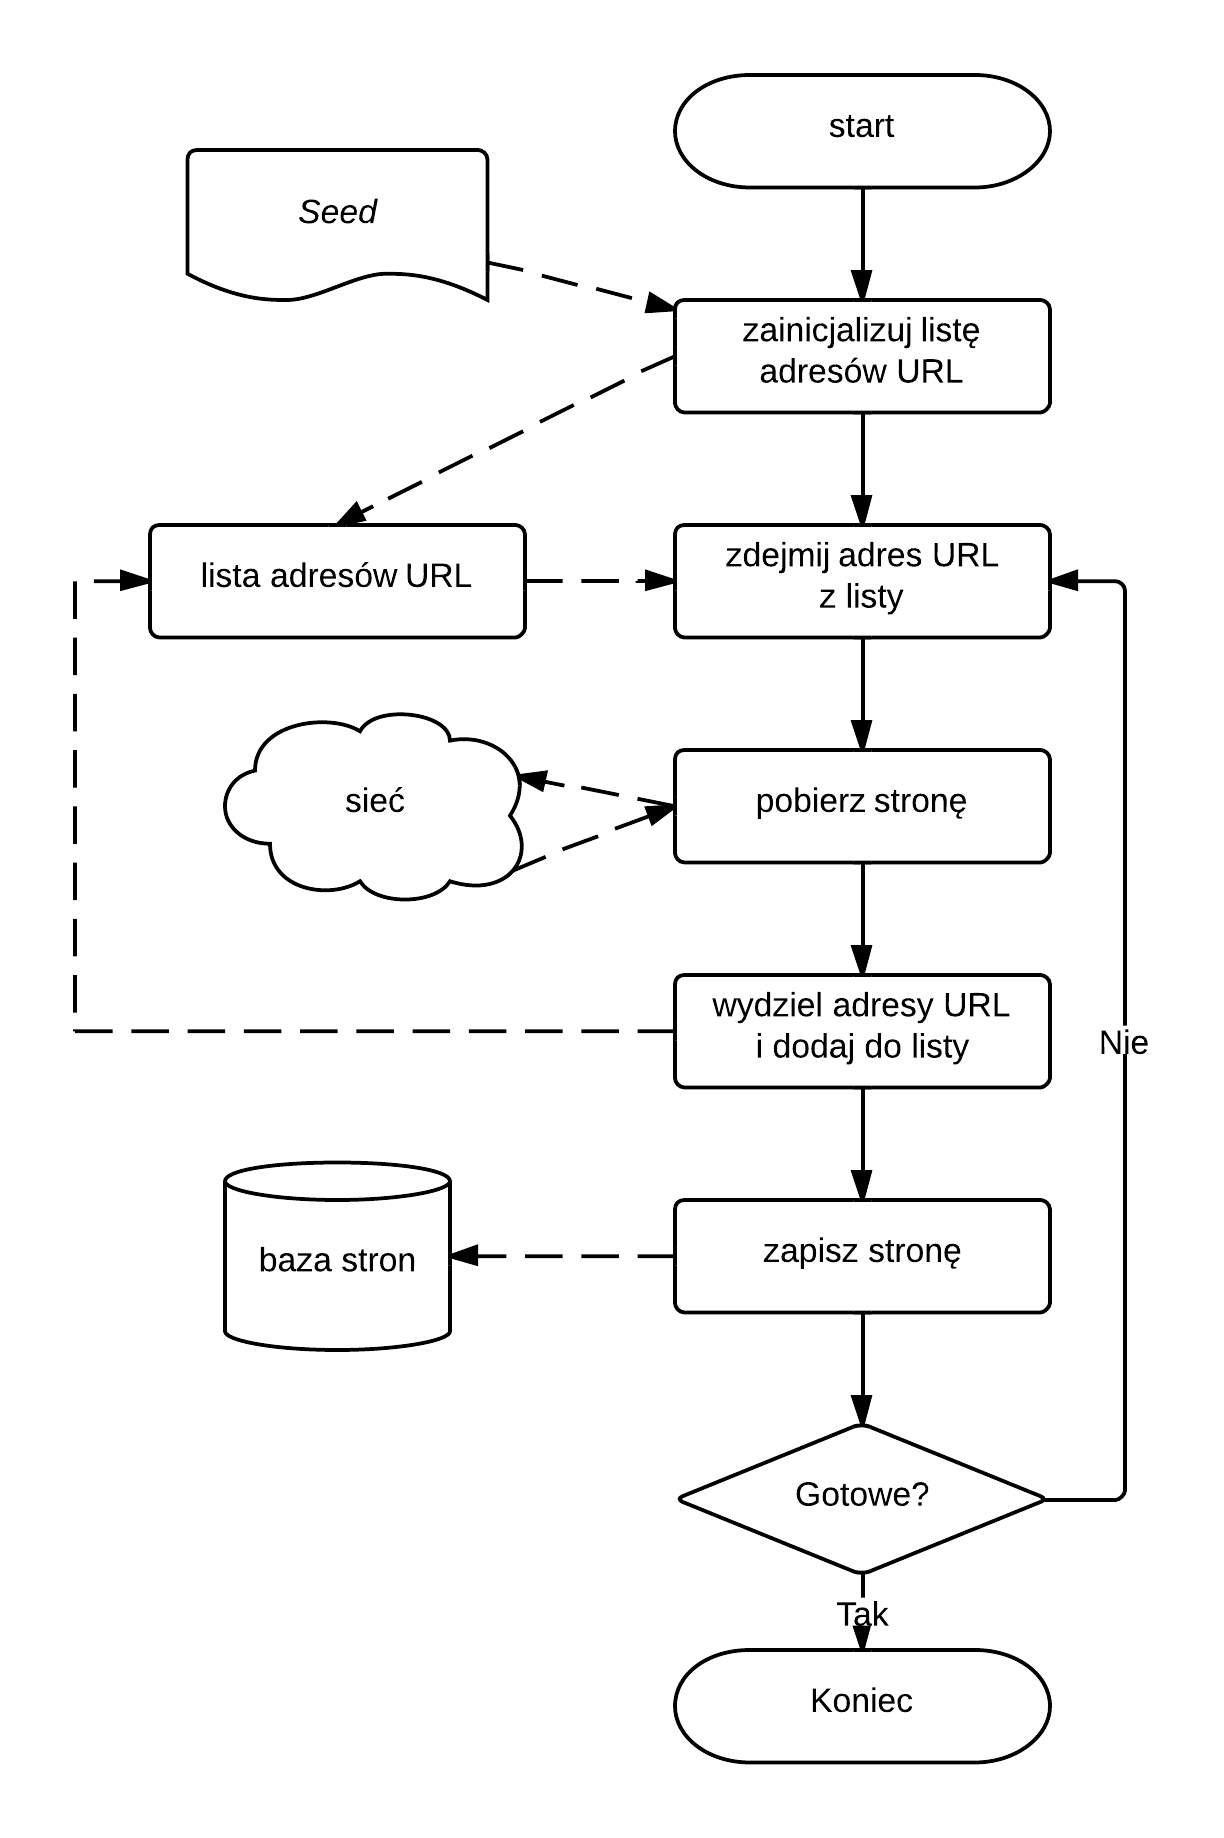
\includegraphics[scale=0.3]{spider_algorithm}
    \caption{Schemat blokowy algorytmu robota internetowego.}
\end{figure}

%%-----------------------------------------------------------------------------------------------------------------------------------------------------

\begin{figure}
    \centering
    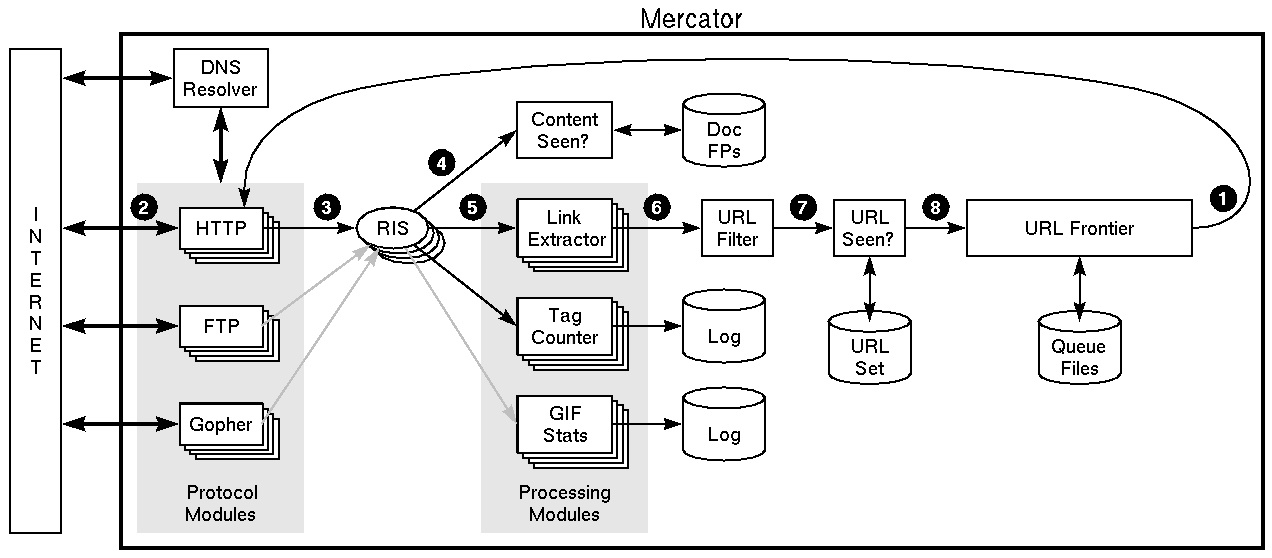
\includegraphics[scale=0.3]{mercator}
    \caption{Schemat crawlera Mercator, implementującego m.in. cache DNS.}
\end{figure}


%%-----------------------------------------------------------------------------------------------------------------------------------------------------

\subsection{Uwagi implementacyjne}
\label{subsec:uwagiImplement}

W związku ze znaczną ilością scenariuszy możliwych do napotkania przy trawersowaniu sieci, jak i dużą ilością danych, która program przetwarza,
stosowane są dodatkowe zabiegi, zwiększające szanse poprawnego działania aplikacji.
\begin{enumerate}
    \item Stosowanie ścisłej kontroli nad ściąganiem stron: ograniczenie czasu trwania połączenia(stosowanie \emph{timeoutów}),
          określenie górnej granicy ilości danych pobieranych z jednej strony(np. do 50 KB), wykrywanie nieskończonych pętli przekierowań,
          logowanie błędów(przekroczenie czasu połączenia, błędne kody odpowiedzi itd.).
    \item Preprocessing pobranych źródeł, mający na celu eliminację częstych błędów występujących na stronach, takich jak np. niedomknięte tagi.
          Wykrycie kodowania i próba jego normalizacji - np. kodowanie wszystkich pobranych źródeł po stronie crawlera w formacie UTF-8.
          Na tym etapie można przeprowadzić również usuwanie słów nie niosących ze sobą istotnych treści(tzw. \emph{stopwords}), takich jak 
          np.~wyrazy ``a'', ``aby'', ``ach'', ``aczkolwiek'', ... itd. Stosowane są również inne formy przetwarzania danych, takie jak
          \emph{lematyzacja}~sprowadzenie do podstawowej formy  gramatycznej i 
          \emph{stemming}~utworzenie tzw. rdzenia słowa, części wspólnej słów niosących podobną informację \cite{lemStem}.
    \item Doprowadzenie linków do postaci kanonicznej. Przede wszystkim należy zapewnić przedstawienie wszystkich URLi w postaci aboslutnej. Ponadto stosowane
          są heurystyki związane np. z usuwaniem numeru portu, o ile figuruje w danym adresie, pozbywaniem się nic nieznaczących sufiksów oznaczających 
          typ dokumentu(np. .html), czy usuwanie tzw. fragmentu - części adresu następującej po znaku ``\#''.
    \item Unikanie tzw. pułapek na pająki (ang. \emph{spide-traps}). \textbf{Pułapka na pająki} to strona, która generuje dynamicznie nieskończenie wiele 
          adresów URL prowadzących do niej samej \cite{spiderTraps}. Przykładem takiej witryny jest aplikacja kalendarza, który generuje linki do stron
          przedstawiających poprzednie lub następne przedziały czasu. Aby uniknąć nieskończonej pętli stosuje się różnego rodzaju heurystyki,
          np.~określa się górny limit ilości pobrań z danej domeny. Ma to jendak negatywny wpływ na aktualność informacji pobieranych ze stron
          o skończonej liczbe odnośników. Wpadnięcie wydajnego crawlera w taką pułapkę powoduje znaczne obciążenie serwerów i może być nawet interpretowane
          przez administratorów strony - pułapki jako atak denial of service \cite[s. 322]{webMining}.
    \item Wprowadzenie wielu wątków/procesów. Jak wspominano wcześniej, czas sekwencyjnego pobierania stron zależy w dużym stopniu od szybkości pobierania
          danych. Również, przy dużej ilości informacji, kosztowne może stać się również zapisaywanie danych na dysku. Jednym ze sposobów skrócenia
          czasu uzyskiwania nowych danych jest zastosowanie wielu równoległych wątków lub procesów, pobierających i przetwarzających dane niezależnie
          od siebie. Następuje wtedy jedynie konieczność synchronizacji dostępu i modyfikacji zarówno listy oczekujących do pobrania adresów URL. Takie
          podejście może w prosty sposób przyspieszyć działanie oprogramowania od 5 do 10 krotnie \cite[s. 323]{webMining}.
          
          Innym ulepszeniem, które może zostać wprowadzone do wielowątkowej architektury, jest pobieranie danych w sposób asynchroniczny. Pozwala to na 
          lepsze wykorzystanie dostępnej przepustowości sieci, niż w przypadku połączeń synchronicznych. Aby ograniczyć czas spędzony na translacji adresów
          URL na adresy IP wprowadza się specjalny serwis wykonujący ją zawczasu dla adresów URL oczekujących w kolejce i cache'ujący rezultaty.
          
\end{enumerate}

%------------------------------------------------------------------------------------------------------------------------------------------------------

\section{Ocena zbioru pobranych stron}
\label{sec:ocenaStron}

Oprócz efektywnego sposobu pobierania informacji z sieci, ważne jest również zrozumienie cech posiadanego zbioru stron internetowych i jego ewaluacja.
W tym przypadku dąży się zarówno do minimalizacji nieaktualnych informacji o witrynach internetowych, jak i do maksymalizacji ilości informacji o stronach
w ogóle. Szczególnie ważne jest szybkie reagowanie na zmiany(dodawanie nowych dokumentów, edycję i usuwanie istniejących), które w wypadku sieci postępują
nadzwyczaj gwałtownie.

\subsection{Świeżość i wiek}
\label{subsec:swiezoscWiek}
Ważną cechą stron jest \textbf{świeżość} (ang. \emph{freshness}) \cite{webMining,webCrawling}. Miara ta jest określona dla pobranej strony \emph{p} w chwili \emph{t} jako
    \begin{equation}
        F_p(t) = 
        \begin{cases}
            1 &\text{  jeżeli } p\text{ jest takie samo, jak lokalna kopia}\\
            0 &\text{ w przeciwnym wypadku}
        \end{cases}
    \end{equation}

Dla tej samej pary można określić również \textbf{wiek} (ang. \emph{age}) \cite{webCrawling}, dany zależnością:
\begin{equation}
        A_p(t) = 
        \begin{cases}
            0 &\text{  jeżeli } p\text{ nie jest modyfikowane w chwili }t\\
            t - \text{czas modyfikacji } p &\text{ w przeciwnym wypadku}
        \end{cases}
    \end{equation}
    
W zależności od podjętych założeń stosuje się różne algorytmy selekcji dokumentów do ponownego odwiedzenia.

%------------------------------------------------------------------------------------------------------------------------------------------------------


\subsection{Algorytmy odświeżania zbioru dokumentów}
\label{sec:odswStron}

Pierwszy z przedstawionych algorytmów dąży do zminiejszenia liczby stron, które moga być nieaktualne. W tym modelu nie ma znaczenia historia historia
zmian zapisanej strony, wszystkie dokumenty odświeżane są z taką samą częstotliwością. Wiąże się to z utrzymywaniem dobrej średniej \textbf{świeżości},
\cite{freshAge} kosztem dopuszczenia możliwości posiadania nieaktualnych wersji pewnych nadzwyczaj często zmieniających się stron. 

Można również stosować inne podejście, które głosi, iż częstotliwość pobierania strony powinna być proporcjonalna do częstotliwości jej zmian w czasie.
Wprawdzie takie podejście sprawdza się dla witryn edytowanych regularnie, jednak nadużywane prowadzi do zbyt częstych, nieprzynoszących nowych informacji
odwiedzin adresów historycznie zmieniających się z dużą częstotliwością. \cite{freshAge}.

Mimo, iż pierwsze podejście jest bliższe optymalnemu, najlepsze rezultaty daje określenie rozkładu prawdopodobieństwa zmian dla poszczególnych witryn i 
dostosowywanie częstotliwości pobierania informacji z tych źródeł do otrzymanych rezultatów \cite{webCrawling}.

%------------------------------------------------------------------------------------------------------------------------------------------------------

\section{Charakterystyka zmian sieci w czase}
\label{sec:zmianySieci}

Poniżej przytoczona zostaje zbiorcza charakterystyka zmian w różnych podzbiorach sieci, uzyskana z \cite{webCrawling}.

\begin{table}[!h]
\caption{Zbiorcze dane dotyczące różnych badań zmian zachodzących w sieci.}
\begin{tabular}{llr}
\hline
\cline{1-2}
Podzbiór    & Obserwacje \\
\hline
360 losowych stron & mediana życia strony\(\approx\) 2.5 roku, \\
&33\% było wciąż dostępnych po 6 latach \\
\hline
500 stron & mediana życia strony \(\approx\) 4.5 roku \\
(arykułów naukowych on-line)&\\
\hline
2 500 stron & średnia długość życia \(\approx\) 50 dni \\
& mediana wieku \(\approx\) 50 dni \\
\hline
4 200 stron & mediana życia strony \(\approx\) 4 lat \\
(artykułów naukowych on-line) &\\
\hline
720 000 stron & średnia długość życia między 60, a 240 dni.\\
& 40\% stron w domenie \texttt{.com} zmienia się codziennie \\
& 50\% stron w domenach \texttt{.gov} i \texttt{.edu} pozostaje bez zmian\\
& przez 4 miesiące \\
\hline
950 000 stron & średni wiek między 4 dniami, a 4 miesiącami.\\
& Strony o dużej iości linków wskazujących na nie\\
& zmieniane częściej.\\
\hline
4 miliony stron & 8\% tygodniowy przyrost nowych stron\\
& 62\% stron tygodniowo dodaje nową treść\\
& 25\% tygodniowy przyrost nowych linków\\
& 80\% zmian jest niewielka\\
\hline
150 milionów stron & w 10 tygodniowym okresie 65\% stron\\
&pozostaje bez zmian\\
& na 30\% stron zachodzą jedynie niewielkie zmiany\\
& duża wariacja dostępności, w zależności od domeny\\
\hline
800 milionów stron & średnia długość życia \(\approx\) 140 dni\\
\hline
\end{tabular} 
\end{table}

Jak widać dynamika zmian w sieci zależy w dużym stopniu od indywidualnych witryn, ich miejsca w grafie oraz
celu, któremu służą. Praktycznie uniemożliwia to skonstruowanie ogólnego algorytmu odświeżającego posiadaną
kolekcję danych w sposób optymalny.

%------------------------------------------------------------------------------------------------------------------------------------------------------

\section{Kwestie etyczne}
\label{sec:etyczne}
Jak wspomniano wcześniej, crawlery używane są w wielu przydatnych zastosowaniach. W związku z tym inwestuje się wiele czasu i pracy w zoptymalizowanie
ich działania, od prostych zabiegów pobierania stron asynchronicznie, po zaawansowane technki modelowania rozkładu prawdopodobieństwa zmian na stronie.
Nie należy jednak zapominać, iż działalność profesjonalnych, bardzo wydajnych robotów internetowych nie pozostaje obojętna dla innych użytkowników 
sieci. Ruch generowany w ten sposób może znacznie obciążać serwery pobieranych stron, powodując kłopoty dla ich administratorów i klientów.
Z tego powodu wprowadzono podstawowe zasady, którymi powinien kierować się każdy projektant oprogramowania trawersującego sieć. W momencie pisania
tej pracy nie mają one podstaw prawnych, ale łamiąc je notorycznie można liczyć się z potępieniem środowiska i poważniejszymi konsekwencjami, jak np.~zablokowaniem
puli adresów IP, z których korzysta nieposłuszny robot.

%------------------------------------------------------------------------------------------------------------------------------------------------------

\subsection{Identyfikacja}
\label{subsec:identyfikacja}

Administratorzy stron zazwyczaj zbierają informacje o ruchu, unikalnych użytkownikach, w których dane o działalności robotów nie są zazwyczaj przydatnymi
informacjami. Aby ułatwić identyfikację robotów, zaleca się umieszczenie w polu nagłówka zapytania HTTP \texttt{user-agent} nazwy crawlera i adresu
strony internetowej zawierającej infomracje o samym robocie oraz dane kontaktowe organizacji odpowiedzialnej za jego działanie.

%------------------------------------------------------------------------------------------------------------------------------------------------------

\subsection{Robot exclusion protocol}
\label{subsec:robotExcl}

W celu zapewnienia kontroli nad zasobami, do których dostęp mają roboty internetowe, wprowadzono protokół wykluczający z indeksowania
(ang. \emph{robot exclusion protocol}). Przyjmuje on formę statycznej strony internetowej serwowanej przez lokalny dla serwisu adres URL 
\url{/robots.txt} \cite{robotsTxt}. Ma ona podobny układ, jak plik \texttt{.txt}, składając się z wielu
następujacych po sobie linii. Każda linia powinna mieć następujący format: \texttt{<pole>:<opcjonalnaspacja><wartosc><opcjonalnaspacja>}.
Wg oficjalnej strony \cite{robotsTxt} \texttt{pole} może być zastąpione przez dwa ciągi znaków:
\begin{itemize}
    \item \texttt{User-agent:} - ciąg znaków odnoszący się do wartość nagłówka \texttt{user-agent} w zapytaniu. Podana dalej wartość identyfikuje
     poszczególne roboty, lub ich grupy. Oznaczanie grup robotów jest możliwe dzięki znakowi szczególnemu ``*'', który oznacza zero lub więcej
     wystąpień dowolnego znaku. Po linii zawierającej to pole następuje jedna lub więcej reguł dostępu do witryny. 
    \item \texttt{Disallow:} - dyrektywa odnosząca się do stron, których crawler nie powinien odwiedzać. Wartość specyfikuje pojedynczy adres URL, lub
     ich grupę wyłączoną z indeksacji.
\end{itemize}
Plik \url{robots.txt} może zawierać również komentarze, rozpoczynane są one znakiem ``\#''. Wszystkie znaki następujące później są ignorowane.
Dodatkowe reguły, respektowane przez niektóre roboty znaleźć można na ich stronach internetowych. Dla przykładu strona \url{https://developers.google.com/webmasters/control-crawl-index/docs/robots_txt}
przybliża sposób parsowania pliku \url{robots.txt} przez robota internetowego firmy Google. Ponadto wprowadza ona możliwość grupowania ciągów identyfikujących
pole \texttt{user-agent} i stosowanie zbioru reguł do całej grupy. Wprowadzona zostaje również dyrektywa \texttt{allow} pozwalająca wyszczególnić
strony, które robot może odwiedziać.

Poniżej znajdują się przykłady zastosowania przedstawionych wcześniej reguł, zaczerpnięte z \cite{robotsTxt}:

\begin{lstlisting}[frame=single]
# robots.txt for http://www.example.com/

User-agent: *
Disallow: /cyberworld/map/
Disallow: /tmp/ # these will soon disappear
Disallow: /bar.pdf
\end{lstlisting}

W tym przypadku żaden robot nie powinien odwiedzać adresu URL zaczynającego się od \url{/cyberworld/map/}, \url{/tmp/} lub \url{/bar.pdf}.

\begin{lstlisting}[frame=single]
User-agent: cybermapper
Disallow:

# go away
User-agent: *
Disallow: /
\end{lstlisting}

Natomiast ten plik pozwala na dostęp do strony tylko robotowi \texttt{cybermapper}.

Ograniczanie dostępu można uzyskać również poprzez umieszczenie w meta tagach HTML klucza \texttt{robots} i wartości
\texttt{noindex} zabraniającej indeksowania danego dokumentu i\textbackslash lub \texttt{nofollow} zabraniającej ściąganie stron linkowanych w 
dokumencie. Natomiast wartość \texttt{nocache} pozwala na pobranie i indeksację dokumentu, jednak nie wyraża zgody na pokazywanie lokalnej kopii
użytkownikom usługi wykorzystującej crawler.

%------------------------------------------------------------------------------------------------------------------------------------------------------

\subsection{Minimalny czas pomiędzy zapytaniami}
\label{subsec:minCzas}
Aby zniwelować obciążenie związane z działalnością crawlerów wprowadza się wymóg minimalnej ilości czasu, która musi upłynąc między dwoma
zapytaniami do tej samej domeny. Spotykane w literaturze propozycje wahają się od 60 do 1 sekundy. Niektóre roboty stosują algorytmy adaptacyjne,
uzależniające odstęp między kolejnymi zapytaniami od szybkości odpowiedzi serwisu \cite{webCrawling}.








%\chapter{Przetwarzanie danych pochodzących z witryn internetowych}
\label{cha:przetwarzanieDanych}



\chapter{Przetwarzanie danych}
\label{cha:budowaGrafu}

Przedstawione w rozdziale \ref{cha:pozyskiwanieTresci} oprogramowanie umożliwia efektywne pobieranie wiadomości z sieci, daje możliwość odświeżania posiadanych informacji
i roszerzania kolekcji dokumentów o nowe pozycje. Rzadko jednak przechowywanie danych jest celem aplikacji. Oprócz programów archiwizujących, zazwyczaj pobranie dokumentu jest pierwszym
etapem algorytmu przetwarzającego dane. Dobrym przykładem jest wyszukiwarka internetowa, w której ważna jest zarówno ilość pobranych stron i ich reprezentatwyność na tle całej sieci, jak
i algorytm oceny przydatności poszczególnych dokumentów.

Jednym z najważniejszych aspektów tworzenia dobrego silnika przetwarzającego dane jest wybór odpowiedniej, przystosowanej do
wykonywanego zadania, struktury danych. Literatura poferuje szeroki wachlarz silników bazodanowych, od relacyjnych, po bazy NoSQL. Niniejsza praca ma na celu przedstawienie wykorzystania
struktur grafowych do przechowywania danych ściągniętych z sieci. W tym rozdziale poruszone zostaną pokrótce zalety przedstawienia danych w postaci grafu i omówiony zostanie pewien 
szczególny rodzaj grafu, jakim jest asocjacyjna grafowa struktura danych(AGDS) \cite[s. 108]{Horzyk}. 

\section{Wykorzystanie grafu jako struktury danych}
\label{section:graf}

%Formalnie, graf jest to uporządkowana para \( G = (V,E)\) zbiorów wierzchołków -\(V\) i krawędzi - \(E\), dla których \(E \subseteq [V]^2 \). Oznacza to, iż 
%czyli elementy \(E\) są 2 - elementowymi podzbiorami \(V\) \cite{teoriaGraf}. 
 
Struktura grafu wyjątkowo dobrze oddaje bezpośrednie relacje pomiędzy elementami w niej zawartymi, ponadto da się przedstawić w prosty i intuicyjny 
sposób. Klasycznymi przykładami problemów matematycznych przedstawiancyh w postaci grafu są np. problem mostów w Królewcu(problem decyzyjny, określający
czy w danym grafie istnieje cykl Eulera), czy problem komiwojażera. Wraz z rozwojem internetowych sieci społecznościowych zaczęto zwracać uwagę na 
możliwości wykorzystania grafów w celu badania sieci, czy przeszukiwania informacji w nich zawartych - przykładem takiego zastosowania jest 
usługa Graph Search udostępniana prez portal Facebook -\url{https://www.facebook.com/about/graphsearch}. Poniżej przedstawione zostaną cechy grafu,
które decydują o jego rosnącej popularności \cite{graphDb}:
\begin{enumerate}
    \item \textbf{Szybkość} - wyszukanie danych o relacjach pojedynczego wierzchołka nie wymaga kosztownych operacji \emph{join} na całych tabelach,
    dostęp do danych jest szybki. Nawet w przypadku wzrostu liczby wierzchołków, czas wykonywania większości zapytań nie zminia się, ponieważ dotyczą
    one jedynie fragmentu bazy.
    \item \textbf{Elastyczność} - graf nie wymaga tak dogłębnego określenia struktury bazy, jak tradycyjna baza relacyjna. Dodawanie nowych relacji, 
    węzłów, czy podgrafów jest stosunkowo proste i nie wymaga migracji. Dzięki temu możliwy jest bardziej dynamiczny rozwój aplikacji opartych o bazy grafowe.
\end{enumerate}

Warto wspomnieć, iż są aplikacje, dla których bazy grafowe są niezastapione, choćby ze względu na ograniczenia szybkości baz relacyjnych. Przykładem na to jest
przytoczone w \cite{neo4jAction} oprogramowanie szukające relacji typu ``znajomy znajomego'' w bazie użytkowników sieci społecznościowych. Dla około~1 000 000
użytkowników posiadających średnio po 50 kontatków, baza grafowa - w tym przypadku Neo4j - okazała się szybsza o kilka rzędów wielkości od tradycyjnej bazy
relacyjnej.

\begin{table}[h!]
\centering
\label{tabela:neo4jAwesome}
\caption{Poszukiwanie ``znajomych znajomych'' w bazie relacyjnej i grafowej}
\begin{tabular}{cccc}
\hline
&  \multicolumn{2}{c}{Czas wykonania [s]} &\\
\cline{2-3}
Zagnieżdżenie & RDBMS & Baza grafowa & Zwrócone rekordy\\
\hline
2 & 0.16 & 0.01 & \(\approx\) 2500 \\
3 & 30.267 & 0.168 & \(\approx\) 110 000\\
4 & 1543.505 & 1.359 & \(\approx\) 600 000\\
5 & nieukończono & 2.132 & \(\approx\) 800 000\\ 
\hline
\end{tabular}
\end{table}


%-----------------------------------------------------------------

\section{Asocjacyjne grafowe struktury danych}
\label{sec:agds}
Często \textbf{asocjacją} (skojarzeniem) nazywa się powiązanie ze sobą dwóch lub więcej zdefiniowanych wcześniej elementów. Zgodnie z \cite[s. 47]{Horzyk} 
tą definicję można rozszerzyć, opierając się na charakterystyce biologicznych organizmów żywych. Zauważono, iż niektóre organizmy mają umiejętność
powiązywania dostepnych dla siebie danych w skomplikowane sieci zależnośc(asocjacji). Do kryteriów, wg których skojarzenia są budowane, należą:
\begin{enumerate}
    \item Miara podobieństwa. 
    \item Odległość w czasie recepcji informacji.
    \item Kontekst, w którym informacje się pojawiły.
\end{enumerate}
W związku z tym, iż organizmy żywe ciągle pozostają pod wieloma względami niedoścignione w wielu dziedzinach(np. jak analiza obrazu, czy mowy, gdy mowa o 
człowieku), postanowiono podjąć próbę kosstrukcji sztucznych systemów asocjacycjnych naśladujących te występujące w naturze.

\subsection{Definicja}
\label{subsec:assocDef}

Poniższe definicje \cite[s. 53-56]{Horzyk} opisują podstawowe elementy systemu asocjacyjnego. Na ich potrzebę można przyjąć, iż ma on ogólną budowę grafu mieszanego,
w którego węzłach umieszczone są sztuczne neurony, a krawędzie odpowiadają synapsom(połączeniom międzyneuronalmy):

\begin{definicja}
    \textbf{Relacją(asocjacyjną)} nazywamy każdą relację pomiędzy obiektami(węzłami) zapamiętywanymi i kojarzonymi ze sobą przez system asocjacyjny.
\end{definicja}

\begin{definicja}
    Powiązania łączące podobne i bliskie dane, ich kombinacje i układy nazywane są \textbf{powiązaniami asocjacyjnego podobieństwa} - \textbf{ASIM}.
\end{definicja}

ASIM ma miejsce wtedy, gdy system przetwarza informacje podobne, jednorodne dane lub ich układy.

\begin{definicja}
    Powiązania łączące dane, ich powiązania i układy, które następują chronologicznie po sobie lub przestrzennie ze sobą sąsiadują są nazywane
    \textbf{powiązaniami asocjacyjnego następstwa} - \textbf{ASEQ}.
\end{definicja}

ASEQ związany jest z powtarzającymi się sekwencjami danych lub danymi pobudzającymi ten sam fragment grafu.

\begin{definicja}
    Powiązania łączące dane, ich kombinacje i układy w taki sposób, że zwykle samodzielnie nie prowadzą do aktywacji neuronów stanowiących węzły
    grafu, lecz stanowią tylko pewien kontekst wspomagający ewentualne wywołanie przyszłych aktywnych reakcji neuronów, wywołanych dopiero na skutek
    następnych procesów skojarzeniowych, nazywa się \textbf{powiązaniami asocjacyjnego kontekstu} - \textbf{ACON}.
\end{definicja}

ACON to powiązanie niemal analogiczne do ASEQ, z tą różnicą, iż nie skutkuje ono od razu aktywacją neuronu, a tylko pełni funkcję wspomagającą.

\begin{definicja}
    Bezpośrednie połączenia od receptorów lub neuronów przekazujących dane wejściowe do neuronu, który reporezentuje niektóre kombinacje lub układy 
    zbudowane z tych danych to \textbf{powiązania asocjacyjnego definiowania} - \textbf{ADEF}.
\end{definicja}

Powstają one w wyniku oddziaływania wielu neuronów, receptorów lub neuronów receptorycznych na ten sam neuron.

\begin{definicja}
    \label{def:agds}
    \textbf{Grafowa asocjacyjna struktura danych AGDS} (ang. \emph{associative graph data structure}) to graf umożliwiający przechowywanie wartości danych
    i ich kombinacji wraz z uproszczoną reprezentacją ich asocjacyjnego podobieństwa(ASIM), asocjacyjnego następstwa(ASEQ) i asocjacyjnego definiowania(ADEF), jakie wystepują między nimi.
\end{definicja}

W zapisie formalnym struktura AGDS jest to uporządkowana siódemka \linebreak \(AGDS = (VV, VR, VS, VC, ESIM, ESEQ, EDEF) \) \cite[s. 109]{Horzyk}, gdzie:

\begin{description}
    \item \(VV\) - zbiór wierzchołków reprezentujących poszczególną wartość (ang. \emph{value vertex}),
    \item \(VR\) - zbiór wierzchołków reprezentujących przedział wartości (ang. \emph{range vertex}),
    \item \(VS\) - zbiór wierzchołków reprezentujących podzbiór wartości (ang. \emph{subset vertex}),
    \item \(VC\) - zbiór wierzchołków reprezentujących kombinację wartości (ang. \emph{combination vertex}),
    \item \(ESIM\) - zbiór krawędzi nieskierowanych, łączących asocjacyjnie podobne wierzchołki,
    \item \(ESEQ\) - zbiór krawędzi skierowanych łączących asocjacyjnie nasępne wierchołki,
    \item \(EDEF\) - zbiór krawędzi dwustronnie skierowanych łączących wierzchołek definiujący z wierzchołkiem definiowanym w taki sposób,
                     iż etykieta (waga) określa przejście od jednego, do drugiego wierzchołka.
\end{description}

Krawędzie dwustronnie skierowane można przedstawić również jako parę krawędzi jednostronnie skierowanych.

Struktura AGDS jest statyczna i stego względu nie można za jej pomocą modelować innych relacji asocjacyjcnych przedstawionych w \cite{Horzyk}.
Typowo dane odwzorowywane są w niej za pomocą węzłów, natomiast krawędzie przedstaiają informację o ich wzajemnym powiązaniu, bazującym np.~na~częstotliwości
występowania. Praca z grafem polega bądź na wykorzystaniu istniejących algorytmów przeszukiwania grafu w celu uzyskania interesujących informacji, bądź
na przekstałceniu struktury AGDS do postaci grafów AANG - \textbf{aktywnych asocjacyjnych grafów neuronowych} i stosowaniu algorytmów asocjacyjnych.
Ważnym założeniem charakterystycznym dla grafów asocjacyjnych jest unikalność informacji przechowywanej w węzłach. 

\subsection{Przedstawienie danych w postaci AGDS}
Na schemacie \ref{graph:relacyjne} przedstawiona jest struktura pewnej relacyjnej bazy danych. Składa się ona z dwóch tabel modelujących relacje:~
użytkowników i prezentów, jakie otrzymali. 

\begin{figure}[!h]
    \centering
    \label{graph:relacyjne}
    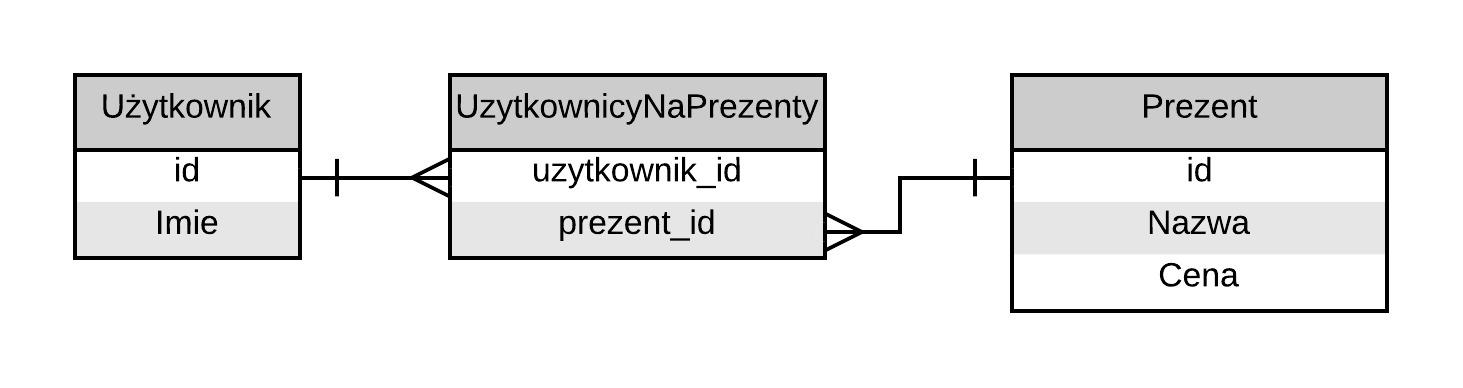
\includegraphics[scale=0.3]{baza_prezenty}
    \caption{Schema relacyjnej bazy danych przedstawiająca użytkowników i prezenty, jakie otrzymali}
\end{figure}

\begin{table}
\centering
\caption{Przykładowe dane}
\begin{tabular}{ccc}

\begin{tabular}[t]{| c | c |}
\hline
id & Imię \\
\hline
1 & Mariusz \\
\hline
2 & Weronika \\
\hline
3 & Bazyl \\
\hline
\end{tabular}
&
\begin{tabular}[t]{| c | c |}
\hline
uzytkownik\_id & prezent\_id \\
\hline
1 & 1 \\
\hline
1 & 2 \\
\hline
2 & 2 \\
\hline
2 & 3 \\
\hline
3 & 4 \\
\hline
3 & 1\\
\hline
3 & 5 \\
\hline
\end{tabular}
&
\begin{tabular}[t]{| c | c | c | }
\hline
id & Nazwa & Cena\\
\hline
1 & Zegarek & 1500 \\
\hline
2 & Łyżwy & 300 \\
\hline
3 & Zegarek & 300 \\
\hline
4 & Łyżwy & 100 \\
\hline
5 & Sweter & 60 \\
\hline
\end{tabular}
\end{tabular}
\end{table}

\begin{table}
\label{tabela:join}
    \centering
    \caption{Tabela joinująca, zaprezentowana w celu zilustrowania danych}
    \begin{tabular}{| c | c | c |}
        \hline
        Imie & Nazwa Prezentu & Cena \\
        \hline
        Mariusz & Zegarek & 1500 \\
        \hline
        Mariusz & Łyżwy & 300 \\
        \hline
        Weronika & Łyżwy & 300 \\
        \hline
        Weronika & Zegarek & 300 \\
        \hline
        Bazyl & Sweter & 60 \\
        \hline
        Bazyl & Zegarek & 1500 \\
        \hline
        Bazyl & Łyżwy & 100 \\
        \hline
    \end{tabular}

\end{table}

W przypadku używania relacyjnej struktury danych, łatwo zauważyc dwa istotne problemy. Gdy wprowadzona zostaje normalizacja, zazwyczaj informacje nie są duplikowane pomiędzy
tabelami, wszystkie zależności wyrażone są w postaci relacji. Jednak operacje na takich zbiorach danych łączą się z koniecznością używania \emph{joinów}, które w wypadku
tabel o wielu rekordach dają duży narzut obliczeniowy(jak przedstawiono na \ref{tabela:neo4jAwesome}). W razie świadomej denormalizacji, jak w przypadku zilustrowanym w tabeli
\ref{tabela:join} mogą występować problemy związane z niespójnością danych. Trundo wprowadzać do takiej struktury zmiany, jest ona podatna na różne anomalie.

Na rysunku \ref{graph:agds} przedstawiony jest ten sam zbiór danych, ale z wykorzystaniem struktur AGDS. Niewątpliwą zaletą takiego przedstawienia jest możliwość natychmiatowego
otrzymania informacji o relacjach zachodzących między poszczególnymi obieketami. Otrzymanie infomracji o liscie prezentów użytkownika, wszystkich użytkownikach posiadających
ten sam prezent, czy średniej cenie prezentu danego typu jest bardzo proste i niewymagające obliczeniowo.

\begin{figure}[!h]
    \label{graph:agds}
    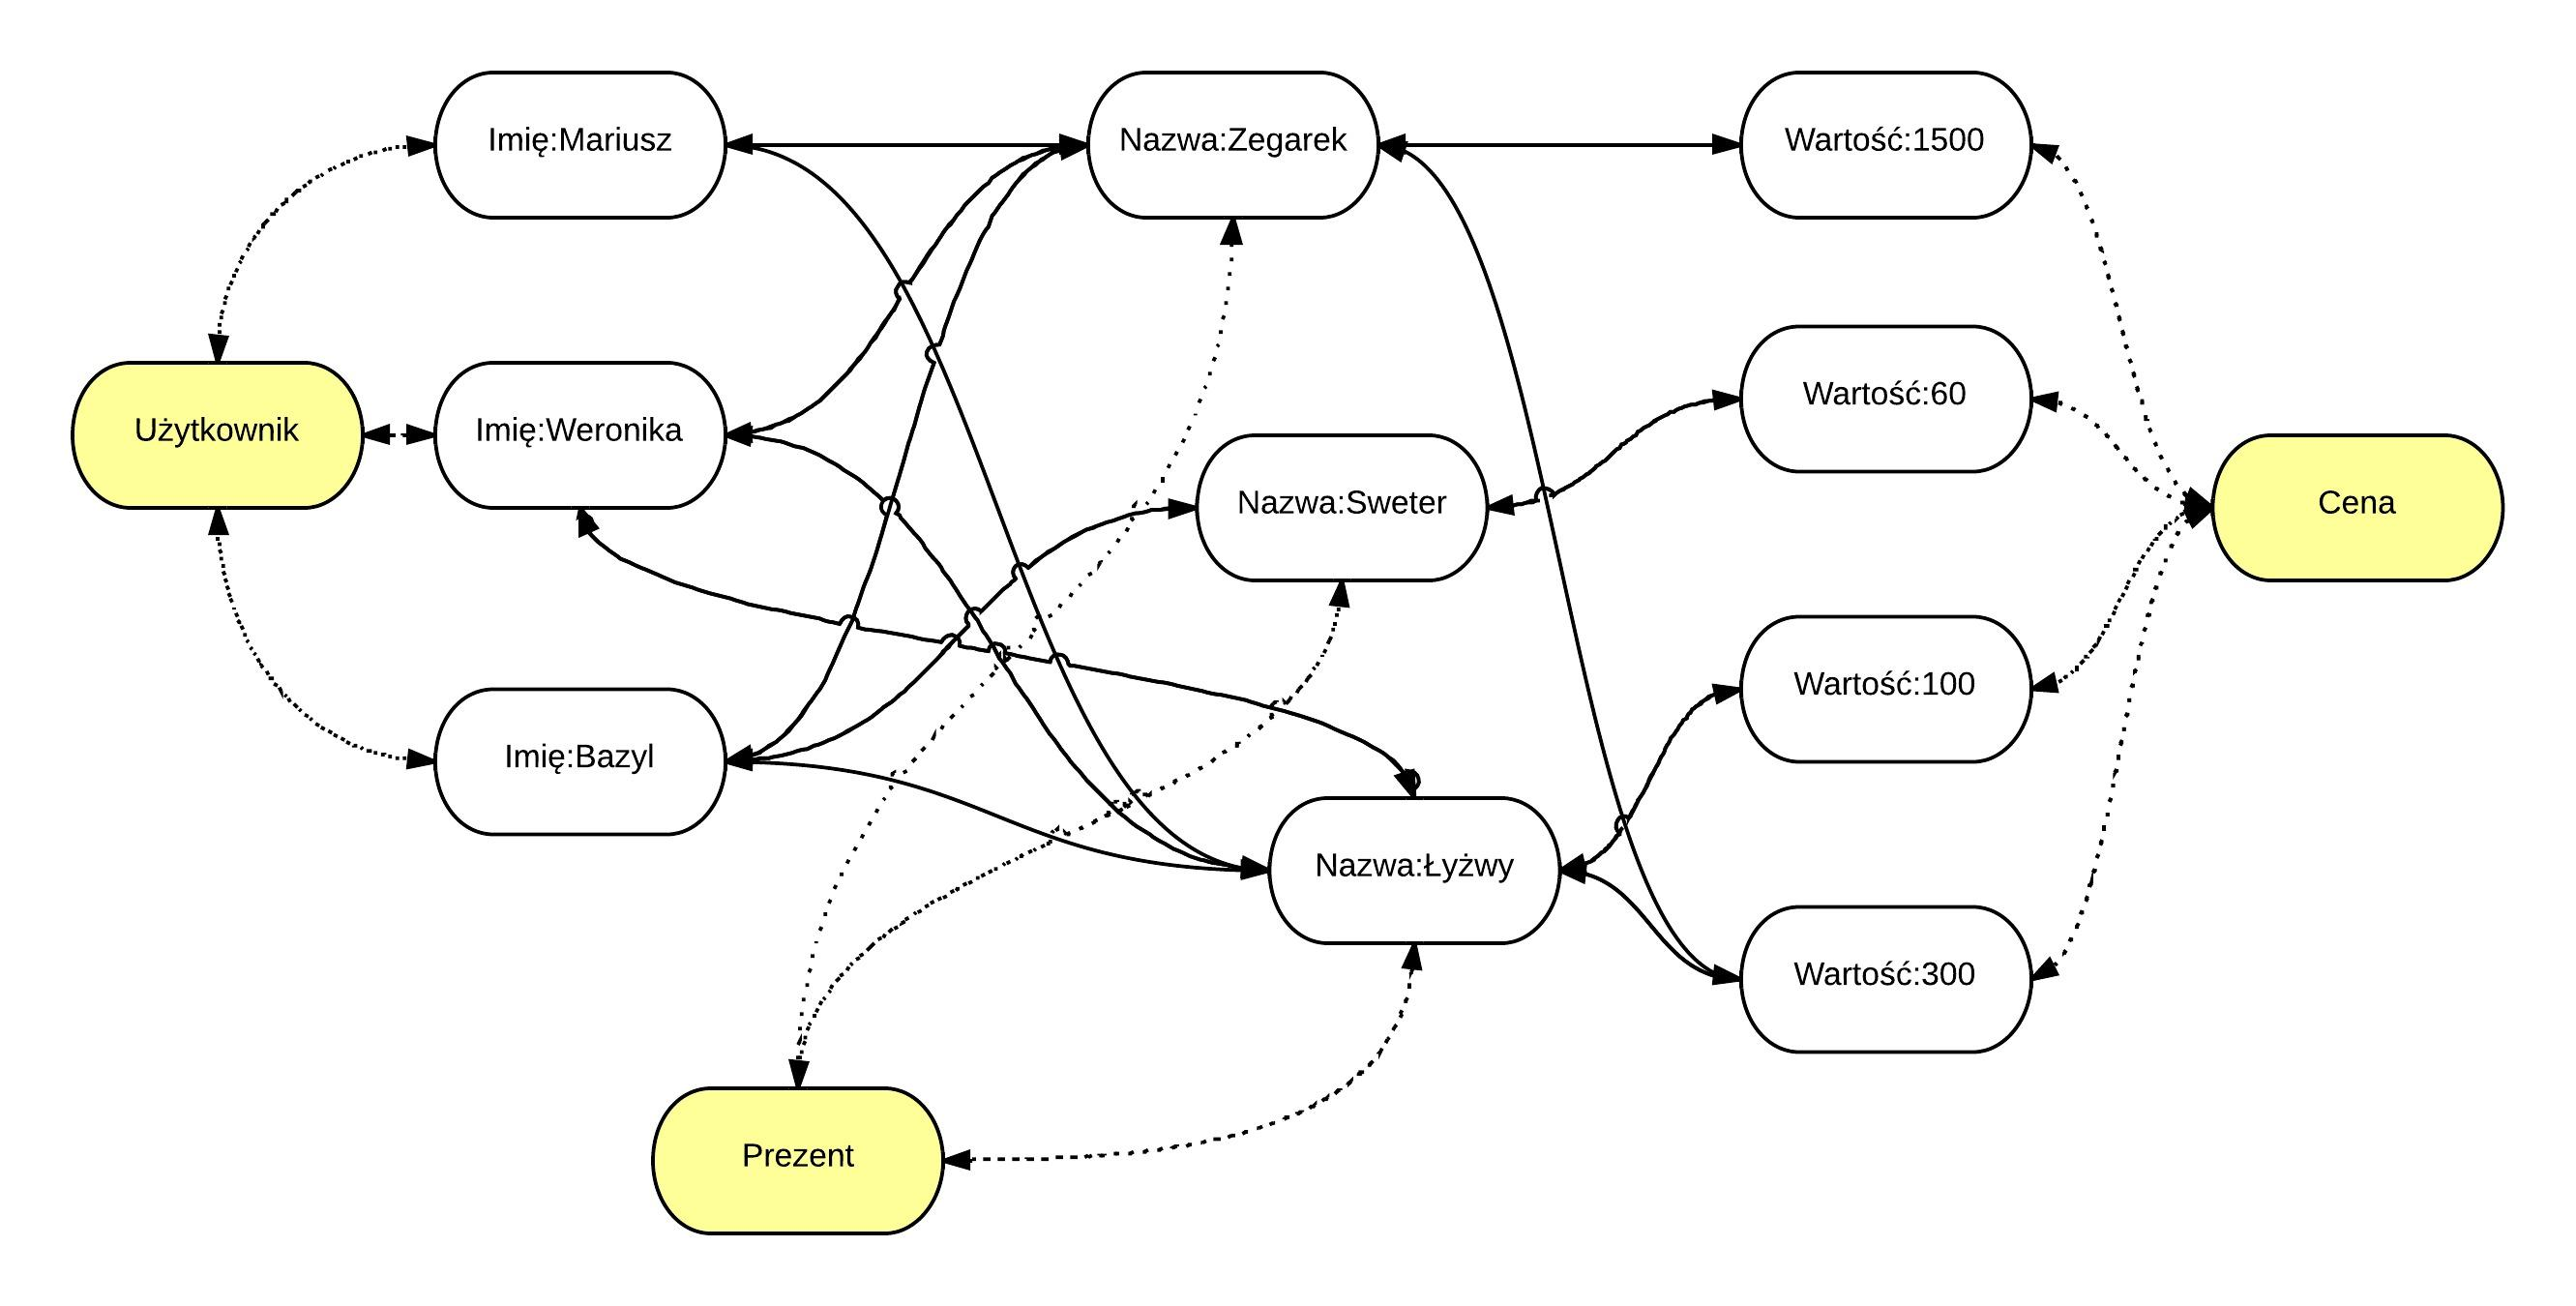
\includegraphics[width=\textwidth]{agds}
    \caption{Graf reprezentujący dane o użytkownikach i prezentach.}
\end{figure}

Zgodnie z \cite[s. 110]{Horzyk} można zauważyć, iż dostęp do każdego obiektu i jego relacji może być zrealizowany w czasie stałym \(O(1)\). W przypadku używania relacyjnych baz danych
z indeksacją za pomocą \emph{B - drzewa} - dostępną w MySQLu, czy PostreSQLu, koszt wyszukiwania wynosi \(O(log n)\). Wprawdzie można stosować index w postaci tablicy z haszowaniem, 
której średni czas dostepu wynosi \(O(1)\), jednak znacznie ogranicza to możliwości operacji na danych posiadających taki klucz.

Rysunek \ref{graph:agds}, dla przejrzystości nie uwzględnia etykietowania krawędzi grafu, ani nie przypisuje im żadnych wartości. Jednak zgodnie z definicją \ref{def:agds} nic nie stoi
na przeszkodzie, aby wprowadzic różne nazwane relacje, posiadające przypisaną im wartość, lub zbiór wartości. Dzięki temu struktury AGDS mogą być używane do przechowywania skomplikowanych,
wielopoziomowych struktur danych. Warto zwrócić uwagę również na łatwość rozszerzania istniejącej struktury o nowe typy węzłów, węzły i łączące je relacje. 

Podsumowując, struktury AGDS mogą być użyte wszędzie tam, gdzie tradycyjne struktury grafowe, dając przy tym nowe możliwości związane z modelowaniem relacji asocjacyjnych.
Szczególnie można wyróżnić następujące zastosowania \cite{Horzyk}:
\begin{itemize}
\item jako alternatywna, asocjacyjna forma reprezentacji i przechowywania danych,
\item do modelowania podstawowych asocjacyjnych relacji pomiędzy danymi,
\item do szybkiego wyszukiwannia powiązanych danych i ich kombinacji,
\item do szybkiego odnajdywania podobieństw, różnic i korelacji,
\item jako pewna forma kompresji danych i ich kombinacji,
\item jako pośrednia forma reprezentacji danych między pasywnym klasycznym oraz alternatywnym asocjacyjnym modelem przetwarzania danych.
\end{itemize}

\section{Aktywne asocjacyjne grafy neuronowe}
\label{sec:AANG}

Jedną z możliwości wykorzystania struktur AGDS jest przekształcenie ich w asocjacyjne grafy neuronowe - \textbf{AANG}. Zazwczyaj AANG nie jest używane \emph{per se}, ale dostoswywane do konkretnych aplikacji, determinując również sposób budowy grafów AGDS.

Założeniem stojącym za grafami AANG jest chęć modelowania biologicznej tkanki mózgowej. Podobnie, jak w przypadku innych sztucznych sieci neuronowych,
konieczne jest stosowanie pewnych uproszczeń, umożliwiających sprawne budowanie, uczenie i ewaluację takch struktur. W tym przypadku nacisk położony
został głównie na modelowanie odpowiedzi neuronu w czasie. Dlatego obliczanie propagacji sybału przez graf AANG polega na symulowaniu, w czasie ciągłym
lub dyskretnym, interakcji neuronów wchodzących w jej skład.

Jako, iż niniejsza praca nie skupia się w znacznym stopniu na symulacji odpowiedzi grafów AANG, wyszczególnione zostaną jedynie najważniejsze cechy neuronów asocjacyjnych.
Pełną definicję można znaleźć w \cite{Horzyk}.

\begin{definicja}
    \textbf{Asocjacyjny model neuronu - ASN} (ang. \emph{associative neuron}) jest modelem funkcjonalnym biologicznego neuronu odwzorowującym jego plastyczne zmiany w czasie oraz
    reaktywne dynamiczne sumowanie ważonych bodźców wejściowych w czasie z uwzględnieniem funkcji relaksacji i refrakcyjności. 
\end{definicja}

W dalszej częsci pracy pojęcia \emph{neuron} i \emph{neuron asocjacyjny} są stosowane zamiennie.

\begin{definicja}
    \textbf{Aktywne asocjacyjne grafy neuronowe} - \textbf{AANG}(ang. \emph{active associative neural graphs}) to pewien rodzaj sieci neuronowych
    opartych na strukturach AGDS zdolnych do aktywnego, asocjacyjnego wiązania danych, ich kombinacji i układów oraz wykonywania na nich neuroobliczeń 
    grafowych. 
\end{definicja}

Grafy AANG posiadają wszystkie zalety i cechy struktur AGDS, przy czym węzły tego grafu zamieniane są w aktywne i warunkowo reaktywe neurony, zaś krawędzie w
 asocjacyjne połączenia pomiędzy nimi. 
 
\section{Neuroasocjacyjne grafy wiedzy ANAKG}
\label{sec:anakg}

Jednym z zastosowań grafów AANG opisanych w sekcji \ref{sec:AANG} jest asocjacyjne modelowanie wiedzy. Sprowadza się ono do przetwarzania pewnego zdefiniowanego typu informacji i 
zapisywania go w postaci grafów AGDS, z możliwością przekształcenia do struktur AANG. Jest to zagadnienie szerokie i nie zostanie dogłębnie zanalizowane. Przytoczona zostanie jedynie
 część pojęć i algorytmów algorytmów, szczególnie związanych z budowaniem struktury AGDS, potrzebna do zrozumienia działania opisywanego projektu.
 
\begin{definicja}
    \label{def:wiedzaSkoj}
    \textbf{Wiedza skojarzeniowa} jest to wiedza fomułowana pod wpływem kombinacji i układów danych oraz ich sekwencji, które można zapisać w postaci \textbf{zbioru sekwencji uczących}
    $\mathbb{S}$.
\end{definicja}

Zbiór sekwencji uczących jest podstawowym nośnikiem wiedzy skojarzeniowej i może być wykorzystany do uczenia specjalnie do tego przygotowanych grafów AANG.

\begin{definicja}
    \label{def:anakg}
    \textbf{Aktywne asocjacyjne grafy wiedzy} - \textbf{ANAKG} (ang. \emph{active neuroassociative knowledge graph}) są pewnym rodzajem grafów AANG o specyficzej postaci dyskretnej
     symulacji czasu aktualizowanego w synchronicznie równoległych krokach dla wszystkich jego elementów \cite[s. 234]{Horzyk}.
\end{definicja}

Budowa grafu ANAKG zaczyna się od zdefiniowania sekwencji uczącej $S \in \mathbb{S}$ i pustego grafu ANAKG. Następnie rozpoczynana jest symulacja dyskretna z krokiem $\Delta t$, 
\begin{equation}
\begin{cases}
    t_0 = 0 \\
    t_i = t_0 + \Delta t * i \\
    t_{max} = t_0 + \Delta t * card(S)
\end{cases}
\end{equation}

 



\chapter{Implementacja}
\label{cha:implementacja}

W tym rozdziale opisana jest realizacja praktyczna projektu. Najpierw omówione zostaną wymagania stawiane całej aplikacji i omówione zostaną podstawowe
założenia związane z jej implementacją. Nastepnie przybliżone zostaną jej poszczególne komponenty.

\section{Wymogi i założenia}
\label{sec:wymogi}

\subsection{Budowa}
\label{subs:budowaAplikacji}

Podstawowym celem projektu jest implementacja oprogramowania pobierającego z podzbioru stron opublikowanych w Internecie dokumenty i przedstawiającego
je w postaci omówionych w Rozdziale \ref{cha:budowaGrafu} asocjacyjnych grafów AGDS. Jest to zadanie wieloetapowe, wymagające następujących komponentów:
\begin{enumerate}
\item Robota dostarczającego dane z sieci. Komponent musi mieć możliwość asynchronicznego pobierania stron WWW, udostępniać API do estrakcji adresów URL z ostatnio
ściągniętych stron spełniających podane warunki oraz implementować \emph{Robots Exclusion Protocol}.
\item Komponentu współpracującego z wyżej opisanym modułem, zapweniającego interfejs umożliwiający zapisywanie danych do zewnętrznej bazy. Umożliwiającego
zapisaywanie kolejnych wersji stron WWW, opisanych \emph{timestampem}.
\item Modułu przetwarzającego wybrane strony WWW przechowywane w zewnętrznej bazie. Powinien on być dawać możliwość parsowania strony HTML i operowania na drzewie DOM.
Powinien mieć możliwość zapisu informacji w formacie JSON, przy zachowaniu budowy umożliwiającej proste rozszerzanie funkcjonalności poprzez dodawanie odpowiednich klas do projektu.
\item Prostego klienta kolejki RabbitMQ, wykonującego RPC z przetworzonymi wcześniej danymi, jako argumentem.
\item Serwera odbierającego wywołania przez kolejkę RabbiMQ, rozpoczynającego konwersję danych do formatu AGDS i zwracającego wynik na kolejkę.
\item Modułu przetwarzającego dane odebrane przez serwer, dzielącego wysyłane strony na sekwencje uczące, umożlwiającego w razie potrzeby proste rozszerzenie funkcjonalności.
\item Silnika asocjacyjnego współpracującego z warstwą zapewniajacą persystencję. Jego jedynym zadaniem jest budowa grafu AGDS zgodnie z założeniami opisanymi w Rozdziale
\ref{cha:budowaGrafu}.
\item Warstwy pośredniczącej pomiędzy aplikacją, a bazami danych. Powinna ona zapisywać logiczną strukutrę grafu w bazie grafowej, a dodatkowe informacje, takie jak
atrybuty poszczególnych węzłów(np. częstość występowania), czy krawędzi(np. waga) przechowywać wlekkiej bazie klucz - wartość. Ważne jest ukreywanie szczegółów implementacyjnych,
zwłaszcza wynikających z używania wielu rodzajów baz danych.
\end{enumerate}

Zanim struktura aplikacji zostanie omówiona w większym detalu, należy opisać platformę, na której powstawała. W związku, z faktem, iż implementacja jest pewnego rodzaju eskperymentem, 
od którego nie wyamga się produkcyjnej sprawności, zaimplementowano ją w języku programowania Ruby. Pozwala on na szybką implementację nowych funkcjonalności, jest w pełni obiektowym i
bardzo elastycznym językiem programowania. Jednak związku z tym, iż Ruby jest językiem interpretowanym i posiada dynamiczne typowanie, zaawansowane możliwości metaprogramowania i 
zapewnia rozbudowane mechanizmy refleksji jego wydajność nie jest duża.
W związku z charakterystyką wybranej platformy program ma szanse działać poprawnie jedynie dla systemów typu Unix(Linux, OS X). Zstosowane zostały dwie wersje interepreterów Ruby'ego:
elementy 1. - 4. wymagają interpretera MRI, wersji conajmniej 2.0.0. Jest to pierwsza implementacja tego języka, napisana w C, większość najważniejszych gemów(bibliotek) jest dostępna 
przede wszystkim dla tej dystrybucji. Natomiast moduły 5. - 8. wymagają użycia alternatywnej implementacji na JVM, o nazwie JRuby. Jest to wymaganie używanej bazy grafowej i jest głównym 
powodem użycia kolejki RabbitMQ do komunikacji między dwoma głównymi częściami aplikacji.

Aplikacja używa 3 baz danych: PostgreSQLa(\url{http://www.postgresql.org/}) do przechowywania ściągniętych stron, Neo4j(\url{http://www.neo4j.org/}) jako bazy grafowej i Redisa(\url{http://redis.io/})
 jako lekkiej bazy klucz - wartość. Wszystkie posiadają biblioteki umożliwiające interakcje z nimi na poziomie obiektów języka, co znacznie ułatwia projektowanie aplikacji. Również każda
 z technologii używanych w projekcie jest technologią \emph{Open Source}.
 
 Każdy komponent posiada testy jednostkowe.

\begin{figure}[!h]
    \centering
    \label{graph:aplikacja}
    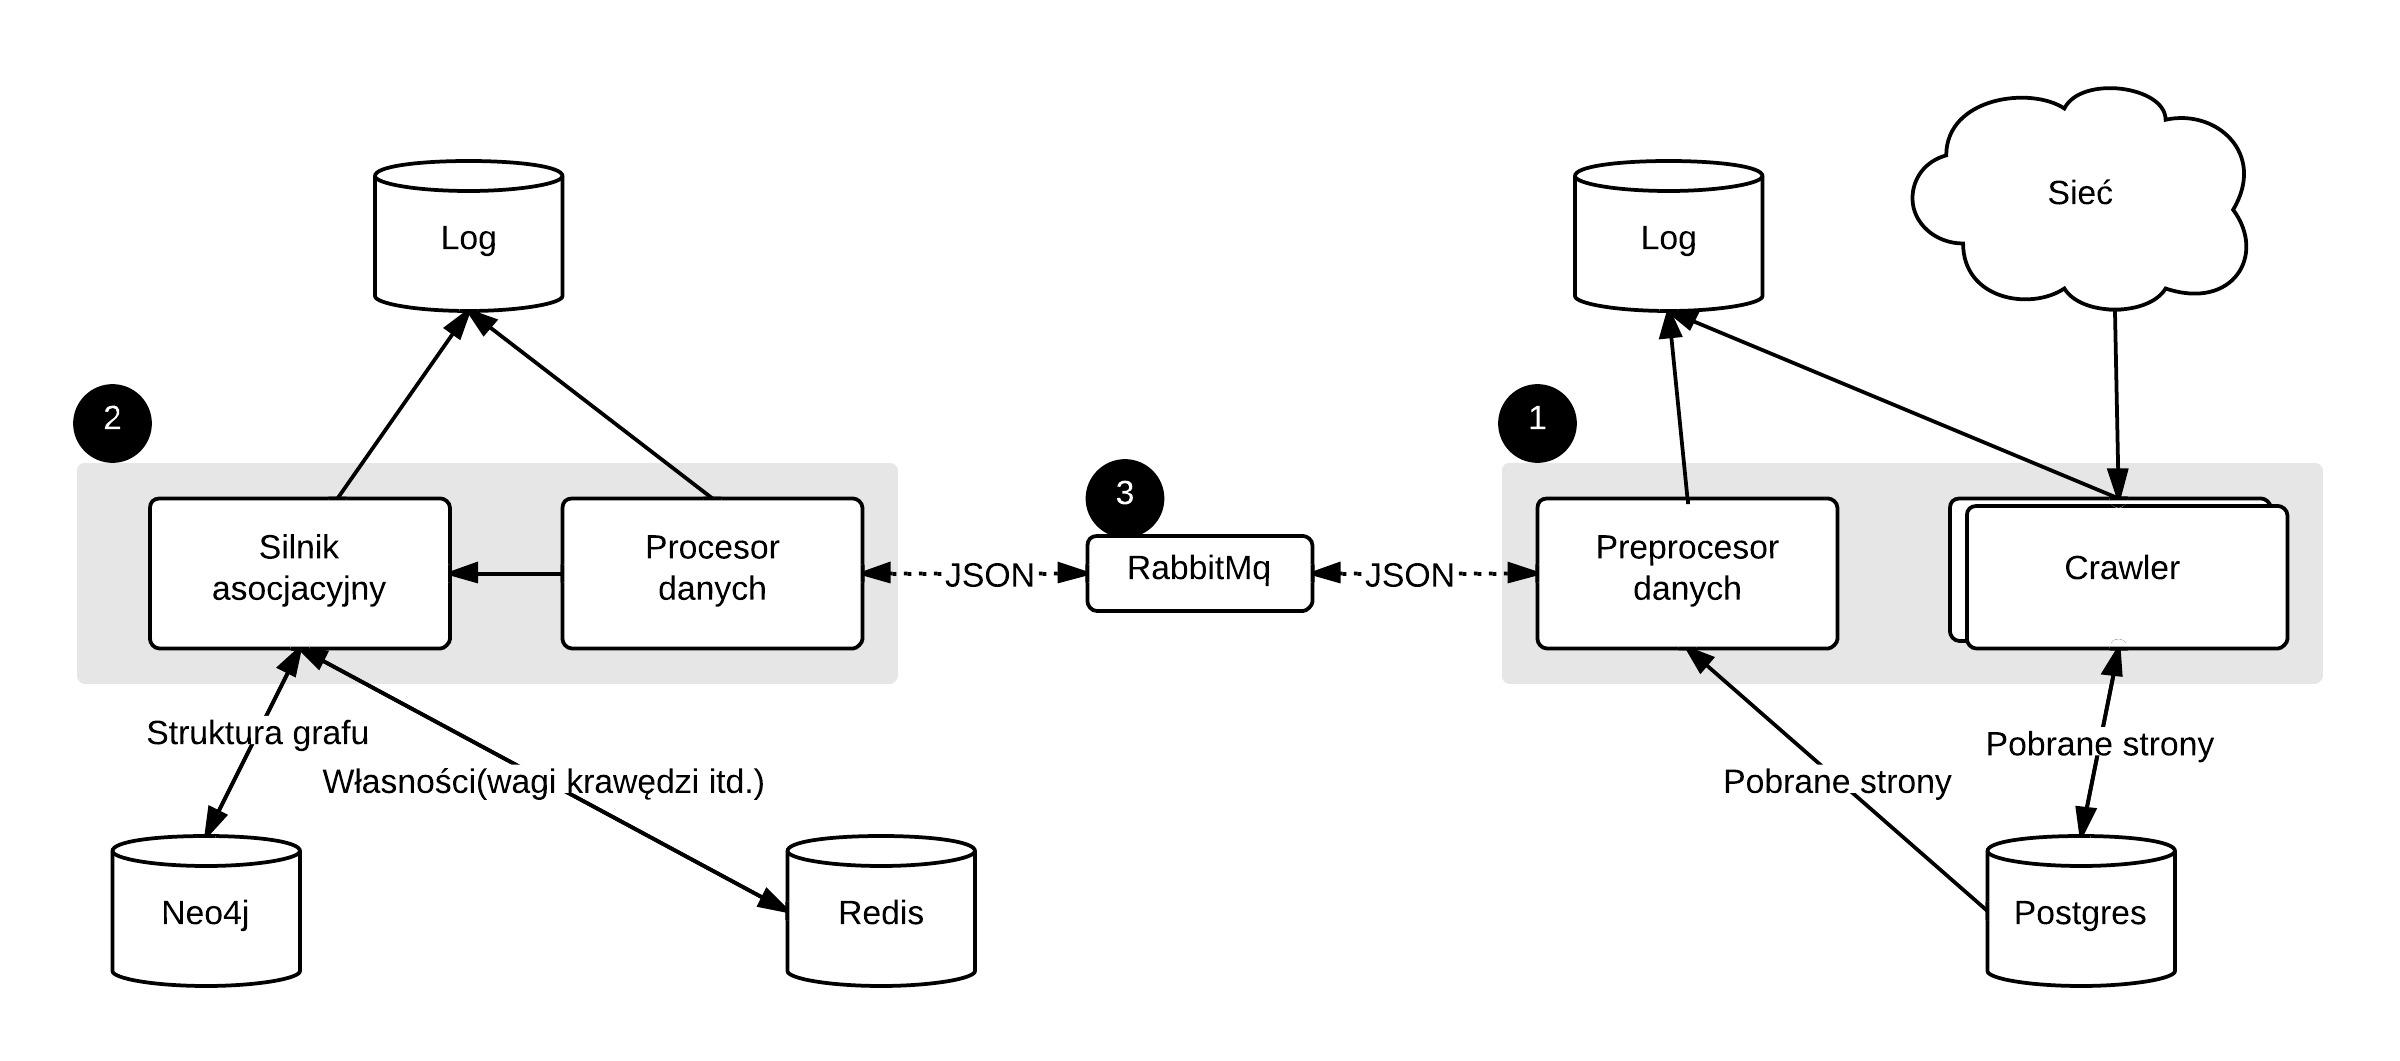
\includegraphics[scale=0.2]{aplikacja}
    \caption{Schemat architektury aplikacji. 1. - część napisana w MRI, 2. - część napisana w JRubym 3. - kolejka}
\end{figure}

\subsection{Wejście/wyjście}
\label{subsec:weWy}

Aplikacja nie posiada interfejsu graficznego. Poszczególne komponenty są wzbudzane z poziomu \emph{shella}, konfiguracja odbywa się poprzez edycję wydzielonych plików konfiguracyjnych, 
opcje podawane przy wykonywaniu skryptów lub zmienne środowiskowe. Celem tej części projektu nie jest serwowanie użytkownikowi informacji, a przedstawianie danych w pewny określonym
formacie, stąd takie ograniczone spektrum możliwości interakcji z aplikacją. Konkretne skrypty uruchamiające aplikacje, opcje ich wywoływania i struktura plików konfiguracyjnych opisana 
jest w dalszej części pracy.

\subsection{Wymagania instalacyjne}
\label{subs:wymaganiaInst}

Aplikacja byla rozwijana i testowana pod systemami typu Unix. Do instalacji i uruchomienia potrzebne są:
\begin{itemize}
\item system kontroli wersji Git (\url{http://git-scm.com/}),
\item Ruby zainstalowany za pomocą systemu kotroli wersji(preferowany rbenv - \url{http://rbenv.org/}),
\item Bundler (\url{http://bundler.io/}) i RubyGems (\url{http://rubygems.org/}),
\item serwer PostgreSQL,
\item baza grafowa Neo4j,
\item serwer Redis.
\end{itemize}

Instrukcje instalacji, konfiguracji i uruchamiania poszczególnych komponentów znajdują się w dalszych częściach pracy.

\section{Opis komponentów 1. - 4.}

Na rysunku \ref{graph:mri} przedstawiony jest detaliczny schemat pierwszych czterech komponentów głównej aplikacji. W istocie tworzą one autonomiczną subaplikację, powiązaną z resztą
komponentów jedynie poprzez kolejkę RabbitMQ. 

\begin{figure}[!h]
    \centering
    \label{graph:mri}
    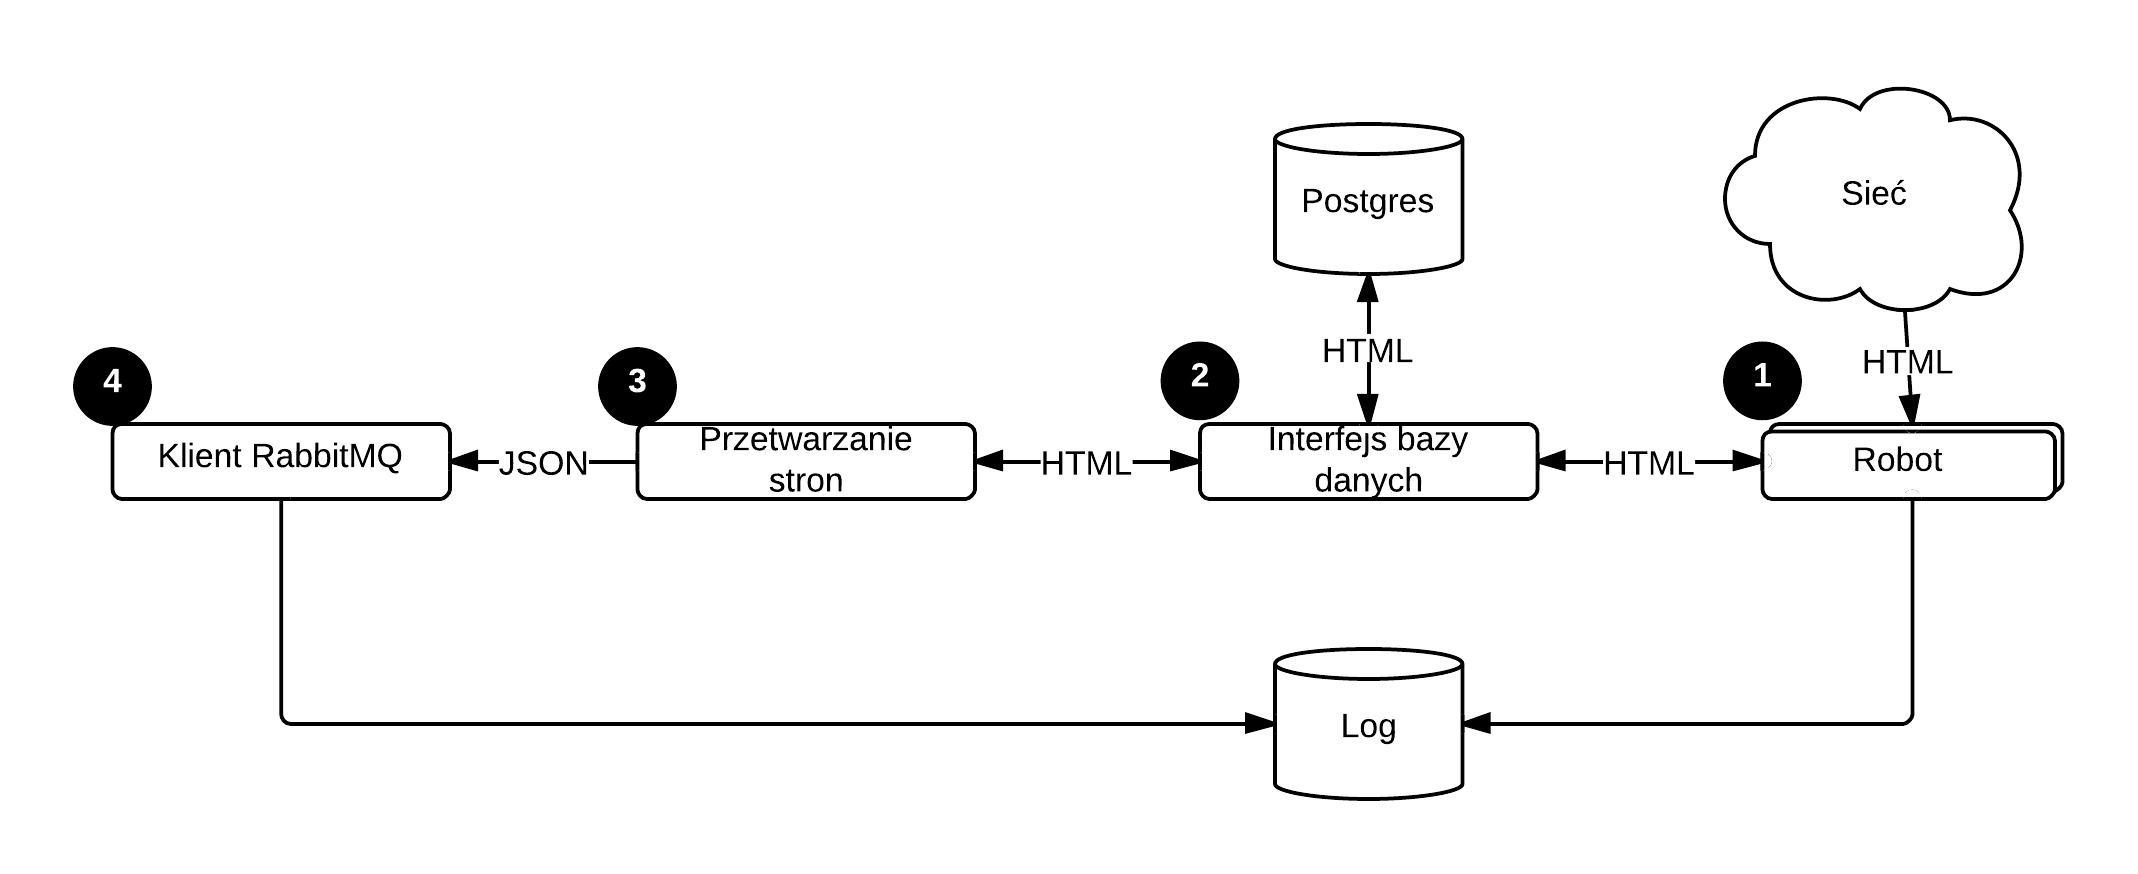
\includegraphics[scale=0.22]{mri}
    \caption{Detaliczny schemat komponentów 1. - 4. Podpisy na strzałkach odnoszą się do formatu, w jakim przedstawiane są strony internetowe na każdym z prezentowanych etapów. }
\end{figure}

\subsection{Konfiguracja}
\label{subs:konfiguracjaMri}

Konfiguracja możliwa jest poprzez dwa pliki znajdujące się w katalogu \texttt{./config}: \texttt{database.yml} i \texttt{config.yml}. Umożliwiają one dostarczenie potrzebnych
informacji pozwalających na połączenie z relacyjną bazą danych, jak i na konfigurację zachowania aplikacji. Poniżej przedstawiony jest listing obu plików 
wraz z wyjaśnieniem dostępnych opcji.

\texttt{database.yml}

\lstset{language=ruby}
\begin{lstlisting}[frame=single]
defaults: &defaults
  adapter: postgresql
  encoding: unicode
  pool: 5
  username: user
  password: pass
  host: localhost

development:
  database: taskmaster_dev
  <<: *defaults
test:
  database: taskmaster_test
  <<: *defaults

\end{lstlisting}

Jest to plik instrumentujący używany w aplikacji ORM - \emph{Active Record}, w celu umożliwienia połączenia z bazą. Konieczne podanie jest typu(\emph{adapter}), 
użytkownika(\emph{user}), hasła(\emph{password}) i lokazlizacji bazy(\emph{host}). Zdefiniowano również specjalne środowisko testowe, dostępne pod luczem \texttt{test}.
Służy ono do definicji bazy powoływanej do egzystencji na czas testów, a następnie bezpowrotnie niszczonej. 

\texttt{config.yml}

\lstset{language=ruby}
\begin{lstlisting}[frame=single]
crawler:
  connections: 20
  fetch_limit: 20
  url_pattern: '\/\/en\.wikipedia\.org\/wiki\/(?!\/|[A-Za-z]+:)'
  starting_page: 'http://en.wikipedia.org/wiki/Main_Page'
  polite: true
  request_gap: 1
queue:
  limit: 50
logger:
  file: 'log/development.log'
  enabled: true

\end{lstlisting}

Plik ten przechowuje informacje konfiguracyjne aplikacji. Kolejno, odpowiadają one za:
\begin{itemize}
\item \texttt{crawler: connections} mówi, ile jednoczesnych asynchronicznych połączeń może wykonywać jeden proces robota.
\item \texttt{crawler: fetch_limit} określa, ile na raz URLi jest wysyłanych do robota w celu ściągnięcia z Internetu. Nie jest t jednoznaczne z parametrem \texttt{connections}, 
w razie wysłania większej ilości adresów URL, niż jest otwieranych połączeń crawler wykona kilka iteracji i zwróci dokumenty odpowiadające wszystkim adresom.
\item \texttt{crawler :starting_page} przechowuje 
\end{itemize}


Łatwo zauważyć, iż dwie pierwsze części tworzą implementację pająka sieciowego, przedstawionego w rozdziale \ref{cha:pozyskiwanieTresci}. Trzeci moduł, 
zaprojektowany jest tak, by umożliwić możliwie najbardziej elastyczny sposób przetwarzania danych, umożliwiający proste dodawnie owych komponentów bez edycji 
istniejącej logiki (zgodnie z regułami programowania obiektowego, szczególnie tzw. \emph{Open - Closed Principle} \cite{ooPrinc}).

Interakcja z modułem opiera się na wywoływaniu w  \emph{shellu} odpowiednich skryptów. 

\chapter{Implementacja}
\label{cha:implementacja}

Zanim struktura aplikacji zostanie omówiona w większym detalu, należy opisać platformę, na której powstawała. W związku z faktem, iż implementacja jest pewnego rodzaju eskperymentem, 
od którego nie wymaga się produkcyjnej sprawności, zaimplementowano ją w języku programowania Ruby. Pozwala on na szybkie wdrażanie nowych funkcjonalności, jest w pełni obiektowym i
bardzo elastycznym językiem programowania. Jednak ponieważ Ruby jest językiem interpretowanym i posiada dynamiczne typowanie, zaawansowane możliwości metaprogramowania raz
zapewnia rozbudowane mechanizmy refleksji jego wydajność nie jest duża.
W związku z charakterystyką wybranej platformy program ma szanse działać poprawnie jedynie dla systemów typu Unix(Linux, OS X). Zastosowane zostały dwie wersje interepreterów Ruby'ego:
elementy 1. - 4. wymagają interpretera MRI, w wersji co najmniej 2.0.0. Jest to podstawowa implementacja tego języka, napisana w C, większość najważniejszych gemów(bibliotek) jest dostępna 
przede wszystkim dla tej dystrybucji. Natomiast moduły 5. - 8. wymagają użycia alternatywnej implementacji na JVM, o nazwie JRuby. Jest to wymaganie wykorzystywanej bazy grafowej Neo4j i dodatkowy powód,
dla którego podzielono aplikację na dwie części.

Aplikacja używa 3 baz danych: PostgreSQLa(\url{http://www.postgresql.org/}) do przechowywania ściągniętych stron, Neo4j(\url{http://www.neo4j.org/}) jako bazy grafowej i Redisa(\url{http://redis.io/})
 jako lekkiej bazy klucz - wartość. Wszystkie posiadają biblioteki umożliwiające interakcję z nimi na poziomie obiektów języka, co znacznie ułatwia projektowanie aplikacji. Również każda
 z technologii używanych w projekcie jest technologią \emph{Open Source}.

\section{Wymagania instalacyjne}
\label{sec:wymaganiaInst}

Aplikacja była rozwijana i testowana pod systemami typu Unix. Do instalacji i uruchomienia potrzebne są:
\begin{itemize}
\item system kontroli wersji Git (\url{http://git-scm.com/}),
\item Ruby zainstalowany za pomocą systemu kotroli wersji(preferowany rbenv - \url{http://rbenv.org/}),
\item Bundler (\url{http://bundler.io/}) i RubyGems (\url{http://rubygems.org/}),
\item serwer PostgreSQL,
\item baza grafowa Neo4j,
\item serwer Redis,
\item kolejka RabbitMQ.
\end{itemize}

Instrukcje instalacji, konfiguracji i uruchamiania poszczególnych komponentów znajdują się w dalszych częściach pracy.

\section{Implementacja komponentów 1. - 4.}

\subsection{Konfiguracja}
\label{subs:konfiguracjaMri}

Konfiguracja możliwa jest poprzez dwa pliki znajdujące się w katalogu \texttt{./config}: \texttt{database.yml} i \texttt{config.yml}. Umożliwiają one dostarczenie potrzebnych
informacji pozwalających na połączenie z relacyjną bazą danych, jak i na konfigurację zachowania aplikacji. Poniżej przedstawiony jest listing obu plików 
wraz z wyjaśnieniem dostępnych opcji.

\texttt{database.yml}

\begin{lstlisting}[frame=single]
defaults: &defaults
  adapter: postgresql
  encoding: unicode
  pool: 5
  username: user
  password: pass
  host: localhost

development:
  database: taskmaster_dev
  <<: *defaults
test:
  database: taskmaster_test
  <<: *defaults

\end{lstlisting}

Jest to plik instrumentujący używany w aplikacji ORM - \emph{Active Record}, w celu umożliwienia połączenia z bazą. Konieczne podanie jest typu(\emph{adapter}), 
użytkownika(\emph{user}), hasła(\emph{password}) i lokalizacji bazy(\emph{host}). Zdefiniowano również specjalne środowisko testowe, dostępne pod kluczem \texttt{test}.
Służy ono do definicji bazy powoływanej do egzystencji na czas testów, a następnie bezpowrotnie niszczonej. 
\newpage

\texttt{config.yml}

\lstset{language=ruby}
\begin{lstlisting}[frame=single]
crawler:
  connections: 20
  fetch_limit: 20
  url_pattern: '\/\/en\.wikipedia\.org\/wiki\/(?!\/|[A-Za-z]+:)'
  starting_page: 'http://en.wikipedia.org/wiki/Main_Page'
queue:
  limit: 50
logger:
  file: 'log/development.log'
  enabled: true

\end{lstlisting}

Plik ten przechowuje informacje konfiguracyjne aplikacji. Kolejno, odpowiadają one za:
\begin{itemize}
\item \texttt{crawler: connections} mówi, ile jednoczesnych asynchronicznych połączeń może wykonywać jeden proces robota.
\item \texttt{crawler: fetch\_limit} określa, ile na raz URLi jest wysyłanych do robota w celu ściągnięcia z Internetu. Nie jest t jednoznaczne z parametrem \texttt{connections}, 
w razie wysłania większej ilości adresów URL, niż jest otwieranych połączeń crawler wykona kilka iteracji i zwróci dokumenty odpowiadające wszystkim adresom.
\item \texttt{crawler: url\_pattern} przechowuje wyrażenie regularne, używane do filtracji adresów URL pobieranych ze stron. Jedynie adresy zgodne z wyrażeniem są zapamiętywane w bazie.
\item \texttt{crawler: starting\_page} podaje stronę startową, od której należy rozpocząć przeglądanie sieci.
\item \texttt{queue: limit} określa ile razy wywołana zostanie procedura przez kolejkę(ile stron zostanie wysłanych) przy jednym wywołaniu skryptu.
\item \texttt{logger: file} przechowuje relatywną wobec folderu projektu ścieżkę logowania.
\item \texttt{logger: enabled} to przełącznik, pozwalający na włąćzanie i wyłącznie loggera.
\end{itemize}

\subsection{Instalacja i uruchomienie}
\label{subs:instalacjaMri}

Po pobraniu repozytoruim i upewnieniu się, że pliki konfiguracyjne zawierają odpowiednie wartości, należy za pomocą \emph{shella} wykonać w katalogu z projektem następujące komendy:
\begin{enumerate}
\item \texttt{\$ bundle} - powoduje ściągnięcie wszystkich zależności,
\item \texttt{\$ rake db:create} - tworzy bazę,
\item \texttt{\$ PROJECT\_ENV=test rake db:create} -tworzy bazę testową,
\item \texttt{\$ rake db:migrate} - migruje bazę do scheme'y wymaganej przez aplikację.
\item \texttt{\$ PROJECT\_ENV=test rake db:migrate} - migruje bazę testową.
\item (opcjonalnie) \texttt{\$ rspec spec} w celu uruchomienia testów.
\end{enumerate}

Aby uruchomić robota internetowego należy w katalogu projektu wykonać polecenie
\texttt{\$ ./download}. W celu uruchomienia klienta kolejki RabbitMQ wystarczy w katalogu projektu wywołać \texttt{\$ ./publish}.
Aplikacja udostępnia również konsolę, umożliwiającą programiście interakcję z załadowanym środowiskiem. Aby z niej korzystać należy w katalogu projektu wywołać polecenie
\texttt{\$ ./console}. 
Zmienna środowiskowa \texttt{PRJOJECT\_ENV} używana jest do kontroli bazy danych, z którą łączy się aplikacja. Domyślnie przyjmuje ona wartość ``development'', a podczas testów
``test''. W celu uruchomienia np. konsoli z bazą testową, należy wywołać \texttt{\$ PROJECT\_ENV=test ./console}.

\section{Implementacja komponentów 5. - 8.}

\subsection{Konfiguracja}
\label{subs:konfiguracjaNeo4j}

Podobnie, jak opisana w sekcji \ref{subs:konfiguracjaMri} część projektu, również komponenty 5. - 8. są konfigurowane za pomocą pliku znajudującego się w katalogu 
\texttt{./config}: \texttt{config.yml}. Odpowiada on za przechowywanie informacji potrzebnych do połaczenia z bazami, lokalizacji plików z logami itd., jak i do 
ustalania parametrów silnika asocjacyjnego. Część opcji dotyczy również silnika symulacyjnego umożliwiającego przeprowadzanie eksperymentów z sieciami ANAKG, jednak
nie jest on bliżej omówiony w niniejszej pracy.

\lstset{language=ruby}
\begin{lstlisting}[frame=single]
payload:
  optional_limit: 2000
  min_word_length: 2
  max_word_length: 25
  max_sentence_length: 4

logger:
  enabled: true
  file: 'log/neo4ruby.log'

redis:
  host: '127.0.0.1'
  port: 6379

search_engine:
  simulation:
    alpha: 0.7
    beta: 0.8
    theta: 1.0
    initial_exc: 0.95
    max_iterations: 10
    min_change_rate: 0.2

  response_scanning:
    limit: 5
    levenshtein_max: 3
    # stopwords after http://www.webconfs.com/stop-words.php
    stopwords_file: 'data/stopwords'

  answer_resolving:
    limit: 10

experiment: 'exp1'

\end{lstlisting}
Poszczególne opcje odpowiadają za:
\begin{itemize}
\item \texttt{payload: optional\_limit} -  maksymalna ilość słów, która jest wprowadzana do bazy grafowej z pojedynczej sekwencji uczącej(pojedynczej strony).
\item \texttt{payload: min\_word\_length} - minimalna długość słowa(słowa krótsze są usuwane z sekwencji uczącej).
\item \texttt{payload: max\_word\_length} - maksymalna długość słowa, j.w.
\item \texttt{payload: max\_sentence\_length} - maksymalna długość zdania. Zdanie w aplikacji jest równoważne kontekstowi opisywanemu w rozdziale \ref{cha:budowaGrafu}.
\item \texttt{logger: enabled} - wł./wył. logowanie.
\item \texttt{logger: file} - lokalizacja pliku z logami.
\item \texttt{redis: } - dane potrzebne do połączenia z Redisem.
\item \texttt{search\_engine: } - parametry symulacji i asocjacyjnej wyszukiwarki internetowej.
\item \texttt{experiment: } - nazwa eksperymentu. Jest to \emph{de facto} ścieżka, w której przechowywane są pliki wbudowanej bazy grafowej. Zmieniając ją, zmienia się
bazę, z którą łączy się aplikacja.
\end{itemize}

\subsection{Instalacja i uruchomienie}
\label{subs:instalacjaMri}

Po pobraniu repozytorum i upewnieniu się, że pliki konfiguracyjne zawierają odpowiednie wartości, należy za pomocą \emph{shella} wykonać następujące komendy:
\begin{enumerate}
\item \texttt{\$ bundle} - powoduje ściągnięcie wszystkich zależności,
\item (opcjonalnie) \texttt{\$ rake test} w celu uruchomienia testów.
\end{enumerate}

Aby uruchomić serwer należy będąc w katalogu aplikacji wywołać polecenie \texttt{\$ ./start}. Przyjumje ono dwa opcjonalne argumenty: \texttt{-e -\--experiment EXP\_NAME} daje możliwość
ręcznego ustawienia bazy, z którą łączy się aplikacja. Zmienna ustawiona w ten sposób nadpisze konfigurację zapisaną w pliku; \texttt{-q -\--queue QUEUE\_NAME} pozwala na zmianę nazwy
kolejki, na której nasłuchuje serwer. Należy jednak wspomnieć, iż ustawienia te były wykorzystywane głównie do rozwoju aplikacji na jej wczesnym stadium, docelowo wszystkie ustawienia
zostaną przeniesione do pliku konfiguracyjnego.

Aplikacja posiada również skrypt ładujący całe środowisko i pozwalający na interaktywną jego eksplorację za pomocą linii komand. Uruchamiany jest on poleceniem \texttt{./console} z
folderu projektu. W razie, gdy istnieje potrzeba połączenia się z inną bazą, niż wyszczególniona w pliku konfiguracyjnym, można użyć opcji \texttt{-e -\--experiment EXP\_NAME}.

\subsection{Struktura przechowywanych informacji}
\label{subs:struktNeo4j}

Z powodów wydajnościowych zdecydowano się na użycie dwóch rodzajów baz: Neo4j odpowiada za przechowywanie struktury grafu,
jego trawersowanie i integralność. To rozwiązanie stosowane jest ze względu na przyjazne API i łatwość integracji z aplikacją. Jednak ze wzgledu na duża ilość wpisów do bazy
podczas tworzenia struktury grafu AGDS(docelowo setki tysięcy stron) oraz konieczność sekwencyjnego budowania grafu, atrybuty elementów grafu, takie jak np. słowa wchodzące
w skład sekwencji uczącej, czy wagi krawędzi sa przechowywane przez prawie cały czas w pamięci programu i zapisywane okresowo w Redisie. Dzięki temu ograniczono znacząco ilość
kosztownych operacji I/O.

\begin{figure}[h!]
    \label{graph:logic_graph}
    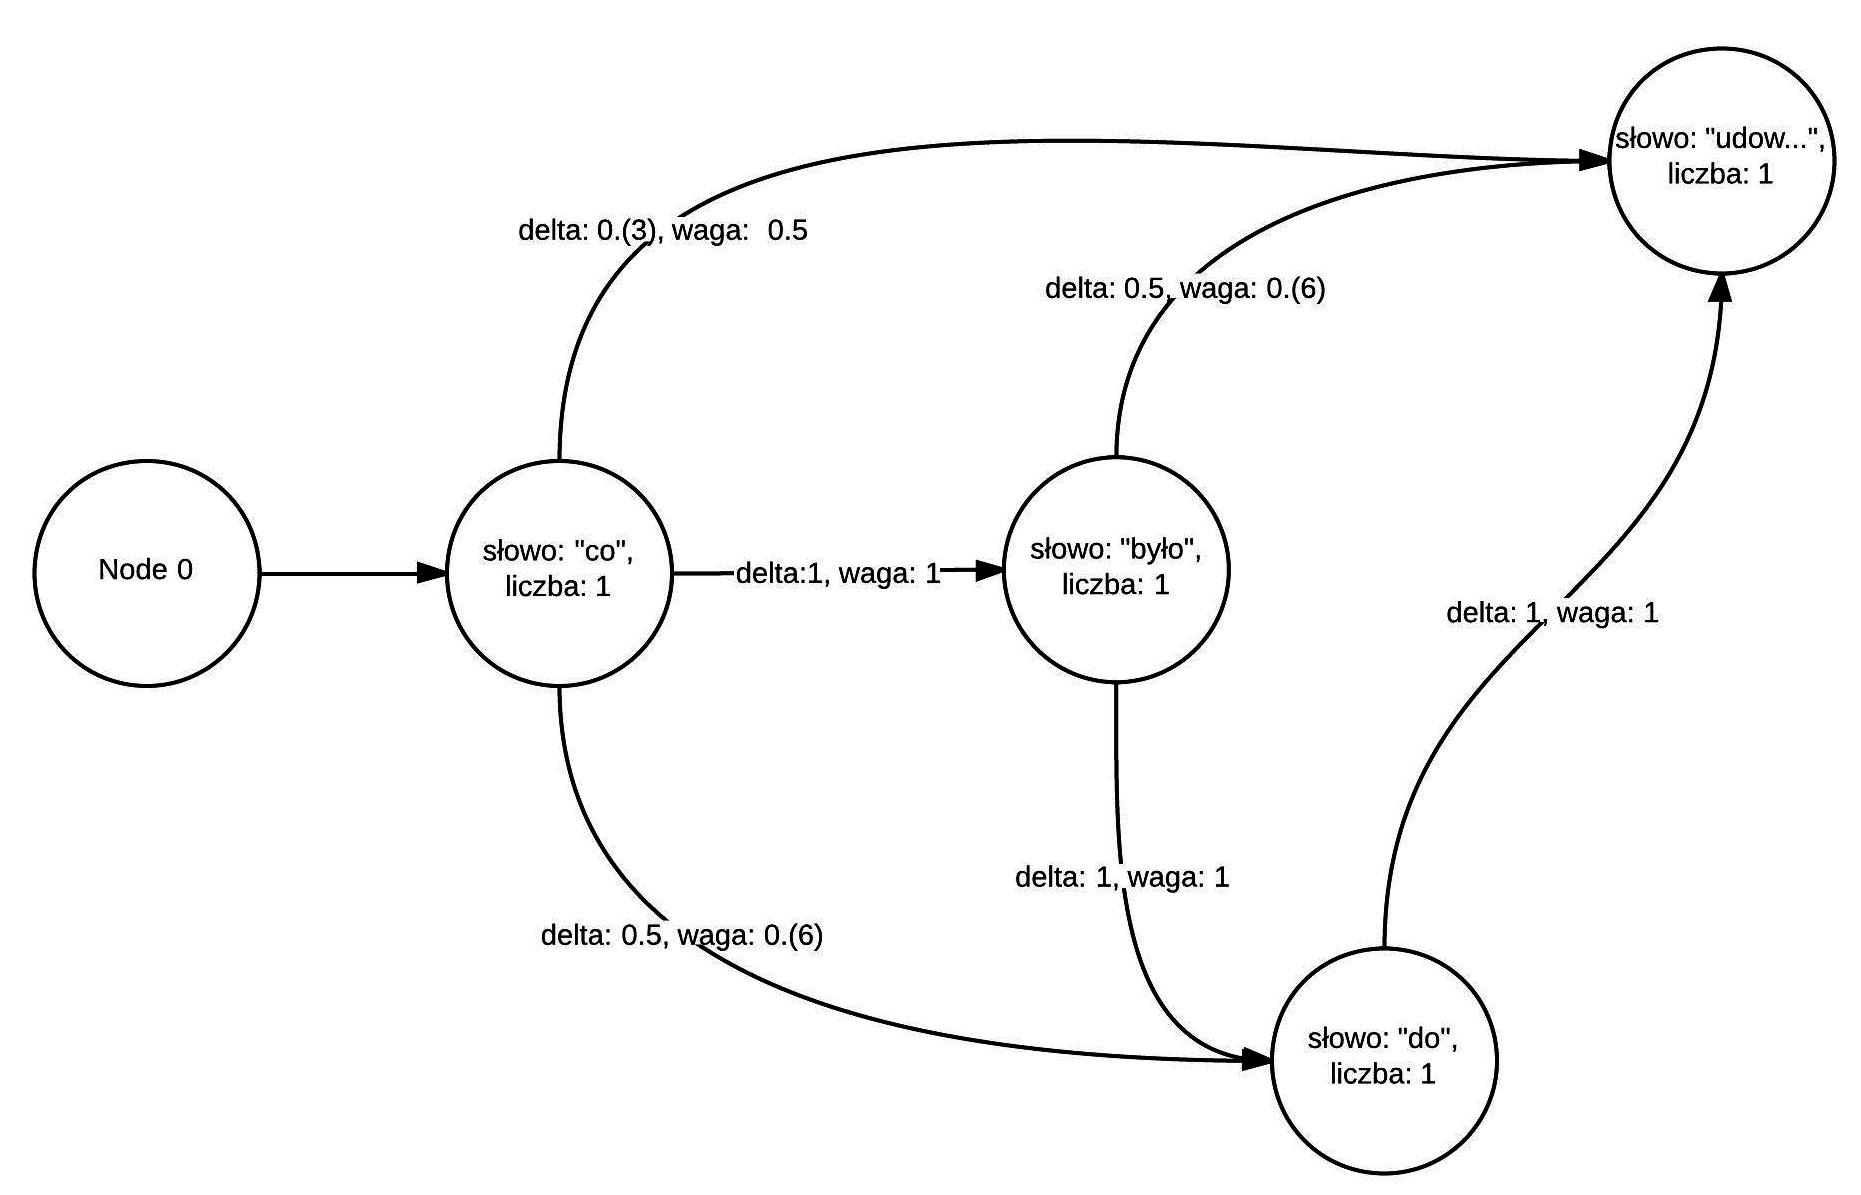
\includegraphics[width=\textwidth]{logic_graph}
    \caption{Przykład reprezentacji sekwencji uczącej w bazie grafowej.}
\end{figure}

Na rysunku \ref{graph:logic_graph} przedstawiona jest logiczna struktura grafu, widziana przez komponenty 5. - 7. Jest to struktura AGDS, powstała na podstawie sekwencji uczącej
$S = \{co, byl{}o, do, udow...\}$. Widoczny jest również domyślny węzeł zerowy(Node 0), obecny w każdej strukturze Neo4j.

\chapter{Testy Oprogramowania}
\label{cha:testy}

Rozdział ten jest poświęcony krótkiemu opisowi testów, którym poddano oprogramowanie w celu sprawdzenia poprawoności działania.
Skupiają się one głównie na poprawności tworzenia struktur AGDS oraz przytaczają wybrane dane dotyczące szybkości tworzenia tych struktur.

\section{Testy poprawności tworzenia struktur AGDS}
\label{sec:testAgds}

Podstawowe test działania oprogramowania opierają się na przykładach zamieszczonych w \cite[s. 228 - 232]{Horzyk}. Przedstawiono tam
kompletny przykład tworzenia struktury AGDS i jej końcowy wygląd. Jeden z przykładów włączony został do zbioru testów automatycznych, zapewniając
w ten sposób częste sprawdzanie najważniejszej funkcjonalności i umożliwiając szybkie wykrywanie błędów.

Test polega na zbudowaniu struktury AGDS modelującej przykładowe sekwencję. Sam proces budowy AGDS, jak i finalny wygląd sieci można znaleźć
w \cite[s.232]{Horzyk}. 

Struktura tworzona jest na podstawie 5 sekwencji uczących, wg wzoru przedstawionego w rozdziale~\ref{cha:budowaGrafu}. 

Sekwencje testowe: $S_1 = \{e1, e2, e3\}, S_2=\{e4, e5, e2, e6\}, S_3 = \{e7, e5, e2, e8\}, S_4 = \{e7, e9, e8\}, S_5=\{e4, e2, e3\}$.

Tabela \ref{tab:test} przedstawia konfrontację wynikowych wag krawędzi AGDS przedstawionych w \cite[s. 232]{Horzyk} i obliczonych przez program.
Widać, iż niewielkie różnice wynikają z dokładności obliczeń numerycznych i nie są związane z niepoprawnością działania implementacji.
\begin{table}[!h]
\centering
\caption{Wyniki tworzenia struktury AGDS dla sekwencji testowych}
\label{tab:test}
\begin{tabular}{ccc}
\hline
Krawędzie  & Waga teoretyczna & Waga wyliczona przez aplikację\\
\hline
\multicolumn{3}{c}{Każda sekwencja jednokrotnie}\\
\hline
$e1 \leadsto e2$ & 1.0  & 1.0\\
$e1 \leadsto e3$ & 0.66  & 0.6666\\
$e2 \leadsto e3$ & 0.66  & 0.6666\\
$e2 \leadsto e6$ & 0.4  & 0.4\\
$e2 \leadsto e8$ & 0.4  & 0.4\\
$e4 \leadsto e2$ & 0.86  & 0.85714\\
$e4 \leadsto e3$ & 0.4  & 0.4\\
$e4 \leadsto e5$ & 0.66  & 0.6666\\
$e4 \leadsto e6$ & 0.29  & 0.2857\\
$e5 \leadsto e2$ & 1.0  & 1.0\\
$e5 \leadsto e6$ & 0.4  & 0.4\\
$e5 \leadsto e8$ & 0.4  & 0.4\\
$e7 \leadsto e2$ & 0.4  & 0.4\\ 
$e7 \leadsto e5$ & 0.66  & 0.6666\\
$e7 \leadsto e8$ & 0.59  & 0.5882\\
$e7 \leadsto e9$ & 0.66  & 0.6666\\
$e9 \leadsto e8$ & 1.0  & 1.0\\
\hline
\multicolumn{3}{c}{$S_1, 5 S_2, S_3, 3 S_4, 2 S_5$}\\
\hline
$e1 \leadsto e2$ & 1.0  & 1.0\\
$e1 \leadsto e3$ & 0.66  & 0.6666\\
$e2 \leadsto e3$ & 0.5  & 0.5\\
$e2 \leadsto e6$ & 0.71  & 0.7142\\
$e2 \leadsto e8$ & 0.2  & 0.4\\
$e4 \leadsto e2$ & 0.78  & 0.7826\\
$e4 \leadsto e3$ & 0.25  & 0.25\\
$e4 \leadsto e5$ & 0.83 & 0.8333\\
$e4 \leadsto e6$ & 0.38  & 0.3846\\
$e5 \leadsto e2$ & 1.0  & 1.0\\
$e5 \leadsto e6$ & 0.53 & 0.5882\\
$e5 \leadsto e8$ & 0.15  & 0.1538\\
$e7 \leadsto e2$ & 0.22  & 0.2222\\ 
$e7 \leadsto e5$ & 0.4  & 0.4\\
$e7 \leadsto e8$ & 0.63  & 0.6285\\
$e7 \leadsto e9$ & 0.86  & 0.8571\\
$e9 \leadsto e8$ & 1.0  & 1.0\\
\end{tabular}
\end{table}


\section{Inne testy i spostrzeżenia}
\label{sec:inneTesty}

Tabela \ref{tab:kontekstTest} ilustruje czas rozbudowy grafu AGDS, w zaeżności od przyjętej długości kontekstu.  Za każdym razem
struktura AGDS budowana była od początku, z wykorzystaniem tej samej sekwencji uczącej, zmieniała się jedynie wartość pola konfiguracyjnego
\texttt{max\_sentence\_length} (kolejno 4, 8 i 12).

\begin{table}[!h]
\centering
\caption{Czas tworzenia grafu AGDS w zależności od wielkości kontekstu}
\label{tab:kontekstTest}
\begin{tabular}{ccc}
\hline
Początkowa ilość węzłów  & Początkowa ilość krawędzi & Czas wstawiania pojedynczej strony[s]\\
\hline
\multicolumn{3}{c}{Maksymalna długość kontekstu 4}\\
\hline
0 & 0 & 3.916 \\
242 & 566 & 18.659 \\
1681 & 8494 & 11.610 \\
1705 & 8573 & 13.768 \\
1915 & 9577 & 16.308 \\
\hline
\multicolumn{3}{c}{Maksymalna długość kontekstu 8}\\
\hline
0 & 0 & 5.57\\
242 & 1246 & 20.464\\
1681 & 12 622 & 24.323\\
1705 & 23 065 & 20.608 \\
1915 & 29 167 & 34.566 \\
\hline
\multicolumn{3}{c}{Maksymalna długość kontekstu 12}\\
\hline
0 & 0 & 6.43 \\
242 & 1854 & 17.539 \\
1681 & 7493 & 24.698 \\
1705 & 23 309 & 38.437 \\
1915 & 33 137 & 42.324 \\
\hline
\end{tabular}
\end{table}

\begin{figure}[!h]
    \centering
    \label{graph:wplyw_kontekstu}
    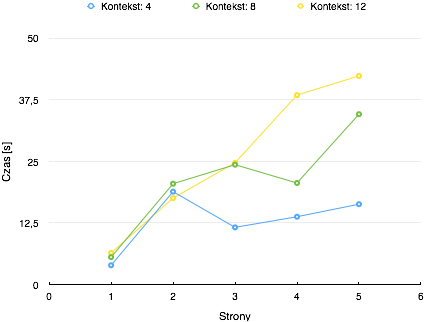
\includegraphics[width=0.8\textwidth]{wplyw_kontekstu}
    \caption{Ilustracja zmiany czasu zapisywania strony w zaleźności od długości kontekstu.}
\end{figure}

\begin{figure}[!h]
    \centering
    \label{graph:wplyw_kontekstu}
    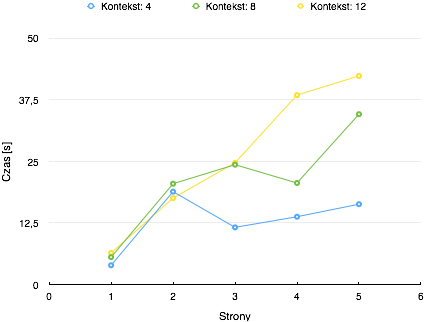
\includegraphics[width=0.8\textwidth]{wplyw_kontekstu}
    \caption{Ilustracja rosnącej liczby krawędzi w zaleźności od długości kontekstu.}
\end{figure}

Jak widać długość kontekstu ma znaczący wpływ na ilość krawędzi grafu, jak i na czas tworzenia struktury. Natomiast ilość węzłów pozostaje bez zmian, co jest zrozumiałe,
ponieważ kontekst określa maksymalną długość połączenia między neuronami, natomiast nie ma wpływu na ich ilość. 

Na rysunku \ref{graph:grafAgds} przedstawiona jest graficzna ilustracja   struktury AGDS zbudowanej na podstawie artykułu znajdującego się pod adresem \url{http://en.wikipedia.org/wiki/Content_(media)}.
Składa się ona z 299 wierzchołków, i 858 krawędzi, kolor i wielkość wierzchołka odpowiadają częstotliowści występowania(i większy, tym częściej występuje. Wierzchołki o tym samym
kolorze występują tą samą liczbę razy). Można zauważyć, iż w tekście znajduje się kilka słów, występujących często i posiadających wiele połączeń. Z analizy grafu dokonanej z poziomu
aplikacji wynika, iż są to w większości słowa z listy \emph{stopwords}, takie jak \emph{the}, \emph{an}, czy \emph{of}(artykuł pisany jest w języku angielskim). Jednak figuruje wśród nich 
również słowo \emph{content}, znajdujące się w tytule artykułu.
Ciekawm zjawiskiem są podgrafy niepołączone z główną strukturą. Przedstawiają one prawdopodobnie definicje uzywające fachowego języka, który nie pojawia się w innych częściach artykułu.

\begin{figure}[!h]
    \centering
    \label{graph:grafAgds}
    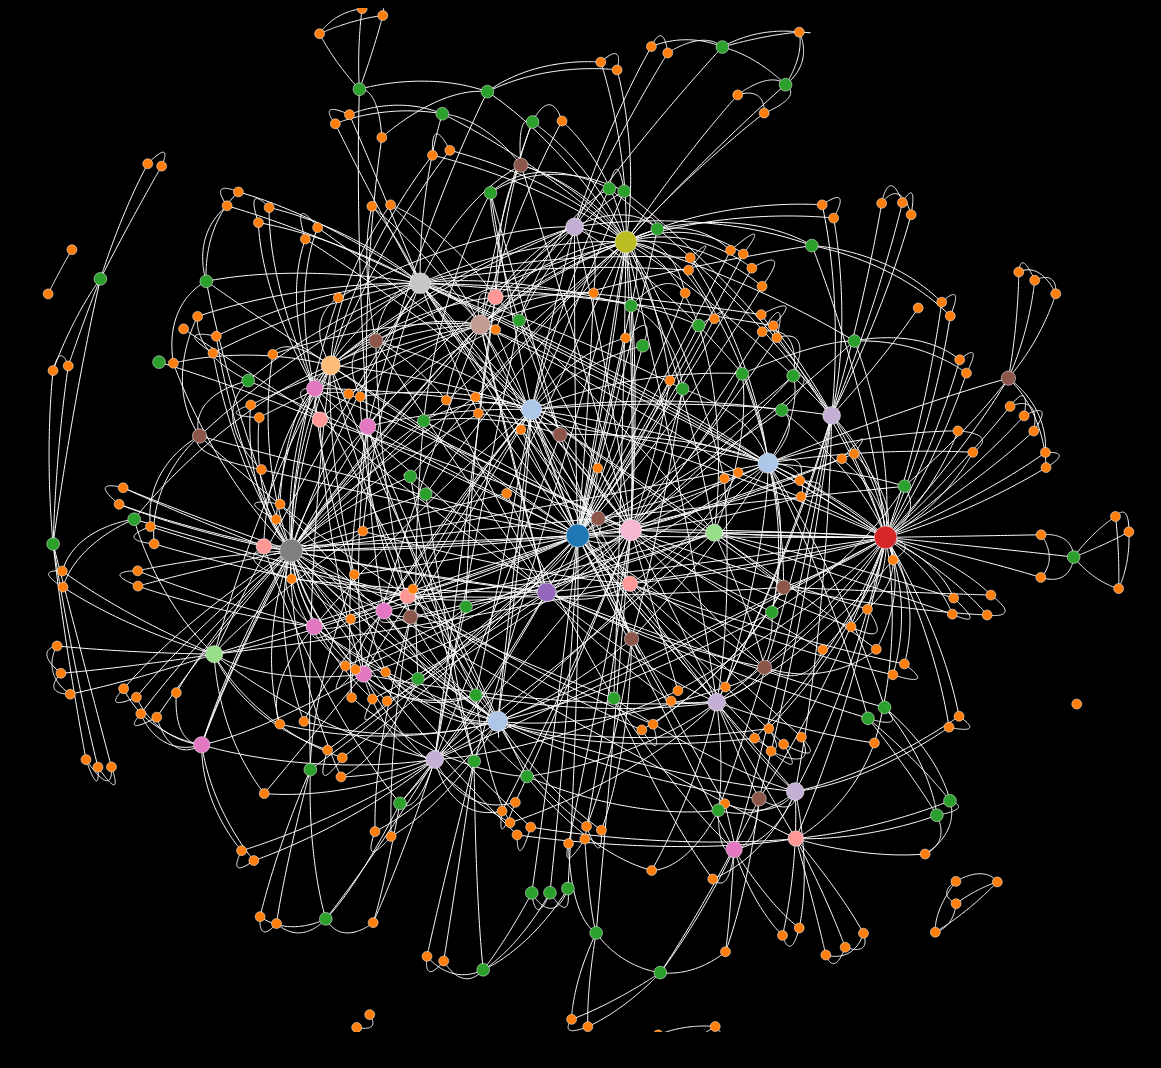
\includegraphics[width=\textwidth]{anakg}
    \caption{Graficzna ilustracja grafu AGDS.}
\end{figure}

%\chapter{Pierwszy dokument}
\label{cha:pierwszyDokument}

W rozdziale tym przedstawiono podstawowe informacje dotyczące struktury prostych plików \LaTeX a. Omówiono również metody kompilacji plików z zastosowaniem programów \emph{latex} oraz \emph{pdflatex}.

%---------------------------------------------------------------------------

\section{Struktura dokumentu}
\label{sec:strukturaDokumentu}

Plik \LaTeX owy jest plikiem tekstowym, który oprócz tekstu zawiera polecenia formatujące ten tekst (analogicznie do języka HTML). Plik składa się z dwóch części:
\begin{enumerate}%[1)]
\item Preambuły -- określającej klasę dokumentu oraz zawierającej m.in. polecenia dołączającej dodatkowe pakiety;

\item Części głównej -- zawierającej zasadniczą treść dokumentu.
\end{enumerate}


\begin{lstlisting}
\documentclass[a4paper,12pt]{article}      % preambuła
\usepackage[polish]{babel}
\usepackage[utf8]{inputenc}
\usepackage[T1]{fontenc}
\usepackage{times}

\begin{document}                           % część główna

\section{Sztuczne życie}

% treść
% ąśężźćńłóĘŚĄŻŹĆŃÓŁ

\end{document}
\end{lstlisting}

Nie ma żadnych przeciwskazań do tworzenia dokumentów w~\LaTeX u w~języku polskim. Plik źródłowy jest zwykłym plikiem tekstowym i~do jego przygotowania można użyć dowolnego edytora tekstów, a~polskie znaki wprowadzać używając prawego klawisza \texttt{Alt}. Jeżeli po kompilacji dokumentu polskie znaki nie są wyświetlane poprawnie, to na 95\% źle określono sposób kodowania znaków (należy zmienić opcje wykorzystywanych pakietów).


%---------------------------------------------------------------------------

\section{Kompilacja}
\label{sec:kompilacja}


Załóżmy, że przygotowany przez nas dokument zapisany jest w pliku \texttt{test.tex}. Kolejno wykonane poniższe polecenia (pod warunkiem, że w pierwszym przypadku nie wykryto błędów i kompilacja zakończyła się sukcesem) pozwalają uzyskać nasz dokument w formacie pdf:
\begin{lstlisting}
latex test.tex
dvips test.dvi -o test.ps
ps2pdf test.ps
\end{lstlisting}
%
lub za pomocą PDF\LaTeX:
\begin{lstlisting}
pdflatex test.tex
\end{lstlisting}

Przy pierwszej kompilacji po zmiane tekstu, dodaniu nowych etykiet itp., \LaTeX~tworzy sobie spis rozdziałów, obrazków, tabel itp., a dopiero przy następnej kompilacji korzysta z tych informacji.

W pierwszym przypadku rysunki powinny być przygotowane w~formacie eps, a~w~drugim w~formacie pdf. Ponadto, jeżeli używamy polecenia \texttt{pdflatex test.tex} można wstawiać grafikę bitową (np. w formacie jpg).



%---------------------------------------------------------------------------

\section{Narzędzia}
\label{sec:narzedzia}


Do przygotowania pliku źródłowego może zostać wykorzystany dowolny edytor tekstowy. Niektóre edytory, np. Emacs, mają wbudowane moduły ułatwiające składanie tekstów w LaTeXu (kolorowanie składni, skrypty kompilacji, itp.).

Jednym z bardziej znanych środowisk do składania dokumentów  \LaTeX a jest {\em Kile}. Aplikacja dostępna jest dla środowiska KDE począwszy od wersji 2. Zawiera edytor z podświetlaną składnią, zestawy poleceń \LaTeX a, zestawy symboli matematycznych, kreatory tabel, macierzy, skrypty kompilujące i konwertujące podpięte są do poleceń w menu aplikacji (i pasków narzędziowych), dostępne jest sprawdzanie pisowni, edytor obsługuje projekty (tzn. dokumenty składające się z~wielu plików), umożliwia przygotowanie i~zarządzanie bibliografią, itp.

Na stronie \underline{\texttt{http://kile.sourceforge.net/screenshots.php}} zamieszczono kilkanaście zrzutów ekranu środowiska {\em Kile}, które warto przejrzeć, by wstępnie zapoznać się z~możliwościami programu.

Bardzo dobrym środowiskiem jest również edytor gEdit z wtyczką obsługującą \LaTeX a. Jest to standardowy edytor środowiska Gnome. Po instalacji wtyczki obsługującej \LaTeX a, edytor nie ustępuje funkcjonalnościom środowisku Kile, a jest zdecydowanie szybszy w działaniu. Lista dostępnych wtyczek dla tego edytora znajduje się pod adresem \underline{\texttt{http://live.gnome.org/Gedit/Plugins}}. Inne polecane wtyczki to: 
\begin{itemize}
\item Edit shortcuts -- definiowanie własnych klawiszy skrótu;
\item Line Tools -- dodatkowe operacje na liniach tekstu;
\item Multi-edit -- możliwość jednoczesnej edycji w wielu miejscach tekstu;
\item Zoom -- zmiana wielkości czcionki edytora z użyciem rolki myszy;
\item Split View -- możliwość podziału okna edytora na 2 części. 
\end{itemize}



%---------------------------------------------------------------------------

\section{Przygotowanie dokumentu}
\label{sec:przygotowanieDokumentu}

Plik źródłowy \LaTeX a jest zwykłym plikiem tekstowym. Przygotowując plik
źródłowy warto wiedzieć o kilku szczegółach:

\begin{itemize}
\item
Poszczególne słowa oddzielamy spacjami, przy czym ilość spacji nie ma znaczenia.
Po kompilacji wielokrotne spacje i tak będą wyglądały jak pojedyncza spacja.
Aby uzyskać {\em twardą spację}, zamiast znaku spacji należy użyć znaku {\em
tyldy}.

\item
Znakiem końca akapitu jest pusta linia (ilość pusty linii nie ma znaczenia), a
nie znaki przejścia do nowej linii.

\item
\LaTeX~sam formatuje tekst. \textbf{Nie starajmy się go poprawiać}, chyba, że
naprawdę wiemy co robimy.
\end{itemize} 





% itd.
% \appendix
% \include{dodatekA}
% \include{dodatekB}
% itd.

\bibliographystyle{plain}
\bibliography{bibliografia}
%\begin{thebibliography}{1}
%
%\bibitem{Dil00}
%A.~Diller.
%\newblock {\em LaTeX wiersz po wierszu}.
%\newblock Wydawnictwo Helion, Gliwice, 2000.
%
%\bibitem{Lam92}
%L.~Lamport.
%\newblock {\em LaTeX system przygotowywania dokumentów}.
%\newblock Wydawnictwo Ariel, Krakow, 1992.
%
%\bibitem{Alvis2011}
%M.~Szpyrka.
%\newblock {\em {On Line Alvis Manual}}.
%\newblock AGH University of Science and Technology, 2011.cccccc
%\newblock \\\texttt{http://fm.ia.agh.edu.pl/alvis:manual}.
%
%\end{thebibliography}

\end{document}
